%! TEX program = xelatex
\documentclass[a4paper,11pt]{article}

% Fonts {{{1
\usepackage{fontspec,amsmath,unicode-math}
\setmainfont[
  Path={/Users/yongrenjie/Library/Fonts/},
  Extension=.ttf,
  UprightFont={*-Regular},
  BoldFont={*-SemiBold},
  ItalicFont={*-Italic},
  BoldItalicFont={*-SemiBoldItalic},
]{SourceSerifPro}
\setmonofont[
  Path={/Users/yongrenjie/Library/Fonts/},
  Scale=MatchLowercase
]{FiraMono-Regular.ttf}
\setmathfont[Scale=1.06]{LibertinusMath-Regular.otf}
\usepackage[final]{microtype}
% }}}1
% Packages and settings {{{1
\usepackage[font=small,labelfont=it,margin=15pt]{caption}
\usepackage{fullpage,parskip,graphicx,float,braket,setspace,subcaption}
\usepackage[svgnames]{xcolor}
\usepackage{chemformula}
\setchemformula{math-scripts=true}
\usepackage[style=chem-acs,subentry,doi]{biblatex}
\addbibresource{genesis.bib}
\graphicspath{{./figures/}}
\usepackage{xurl}   % must be after biblatex
\usepackage[
  mode=match,
  propagate-math-font=true,
  reset-math-version=false,
  reset-text-family=false,
  reset-text-series=false,
  text-family-to-math=true,
  text-series-to-math=true
]{siunitx}
\usepackage[symbol]{footmisc}
\usepackage{hyperref}
\hypersetup{
    colorlinks,
    linkcolor={red!50!black},
    citecolor={blue!60!black},
    urlcolor={blue!80!black}
}
% \makeatletter
% \def\HyColor@@@@UseColor#1\@nil{\addfontfeatures{Color=#1}}
% \makeatother
\usepackage[capitalise,noabbrev]{cleveref}

\usepackage{usebib}
\newbibfield{entryset}
\bibinput{genesis}

\onehalfspacing
\DeclareSIUnit{\molar}{\textsc{m}}
\DeclareSIUnit{\ppm}{ppm}
% }}}1
% Newcommands {{{1 
\newcommand{\genesistitle}{Modular pulse programme generation for NOAH supersequences}
\newcommand{\crl}{Chemistry Research Laboratory, Department of Chemistry, University of Oxford, Mansfield Road, Oxford, OX1 3TA, U.K.}
\newcommand{\brukeruk}{Bruker UK Ltd., Banner Lane, Coventry, CV4 9GH, U.K.}
\newcommand{\proton}{\ch{^{1}H}}
\newcommand{\carbon}{\ch{^{13}C}}
\newcommand{\nitrogen}{\ch{^{15}N}}
\newcommand{\CH}{\carbon{}--\proton{}}
\newcommand{\HC}{\proton{}--\carbon{}}
\newcommand{\NH}{\nitrogen{}--\proton{}}
\newcommand{\HN}{\proton{}--\nitrogen{}}
\newcommand{\HH}{\proton{}--\proton{}}
\newcommand{\todo}[1]{\textcolor{Crimson}{#1}}
\newcommand{\changed}[1]{\textcolor{DodgerBlue}{#1}}
\newcommand{\autociteset}[1]{\autocite{\usebibentry{#1}{entryset}}}
\newcommand{\onejch}{{}^1\!J_{\ch{CH}}}
\newcommand{\njch}{{}^n\!J_{\ch{CH}}}
\newcommand{\onejnh}{{}^1\!J_{\ch{NH}}}
\newcommand{\onejxh}{{}^1\!J_{\ch{XH}}}
\newcommand{\theurl}{\url{https://nmr-genesis.co.uk}}
\newcommand*{\andro}{Spectra were obtained on a \SI{700}{\MHz} Bruker AV III equipped with a TCI H/C/N cryoprobe; the sample used was \SI{40}{\milli\molar} andrographolide in DMSO-\(d_6\).}
\newcommand*{\grami}{Spectra were obtained on a \SI{700}{\MHz} Bruker AV III equipped with a TCI H/C/N cryoprobe; the sample used was \SI{40}{\milli\molar} gramicidin in DMSO-\(d_6\).}
\newcommand*{\zolmi}{Spectra were obtained on a \SI{700}{\MHz} Bruker AV III equipped with a TCI H/C/N cryoprobe; the sample used was \SI{50}{\milli\molar} zolmitriptan in DMSO-\(d_6\).}
% }}}1
% Counters for the combinatorics {{{1
\newcount\nmoda
\newcount\nmodb
\newcount\nmodc
\newcount\nmodd
\newcount\nmode
\newcount\nmoddup
\newcount\nmoddoublehom
\nmoda=2
\nmodb=3
\nmodc=5
\nmodd=9
\nmode=19
\nmoddoublehom=6
\nmoddup=\numexpr(\nmodc-1)
\newcommand{\ee}[1]{\the\numexpr#1\relax}
% }}}1

\begin{document}
\begin{refsection}

\begin{center}   % Front matter
    \textbf{\Large \genesistitle{}}

    \vspace{0.2cm}

    Jonathan R.\ J.\ Yong,\textsuperscript{1} {\=E}riks Kup{\v{c}}e,\textsuperscript{2} Tim D. W. Claridge\textsuperscript{1,*}

    \vspace{0.2cm}

    \textsuperscript{1} \textit{\crl{}}

    \textsuperscript{2} \textit{\brukeruk{}}

    \textsuperscript{*} \texttt{tim.claridge@chem.ox.ac.uk}

    \vspace{0.5cm} \hrule
\end{center}

\section*{Abstract}

\textit{(132 words)}

NOAH (NMR by Ordered Acquisition using \proton{}-detection) supersequences allow multiple 2D NMR datasets to be acquired in greatly reduced experiment durations through the elision of recovery delays.
In NOAH experiments, up to five ``modules'' can be combined, which means that there is a very large number of plausible supersequences (over 4000).
This renders the traditional method of pulse programme construction by hand wholly inadequate.
We introduce here a tool named GENESIS (GENEration of Supersequences In Silico), available via \theurl{}, which programmatically generates arbitrary NOAH supersequences compatible with Bruker spectrometers.
This not only allows users to obtain customised supersequences for specific applications, but also enables us to rapidly and effortlessly disseminate new NOAH modules (e.g.\ PSYCHE, 2D J) as well as improvements to existing modules (e.g.\ \CH{} HMBC, \NH{} HMQC).

\section{Introduction}

The acceleration of NMR data acquisition has in recent years proven a fruitful area for NMR pulse sequence and method development, particularly for \(n\)-dimensional (\(n\)D) NMR where raw data are acquired as a series of time increments.
Developments in this area include (but are not limited to) ultrafast NMR\autociteset{ultrafast}, non-uniform sampling (NUS)\autociteset{nus}, multiple-FID experiments\autociteset{multifid}, and the shortening or elision of recovery delays\autociteset{reducedd1}.
NOAH (NMR by Ordered Acquisition using \proton{}-detection) experiments\autociteset{noah}, which fall under the last two categories, consist of a series of multiple 2D experiments (``modules''), combined into one single ``supersequence'' which uses only one recovery delay for all modules.
This provides substantial (up to \(4\times\)) time savings compared to conventional acquisition, in which one recovery delay is used for each module (\cref{fig:noah_diagram}).

\begin{figure}
    \centering
    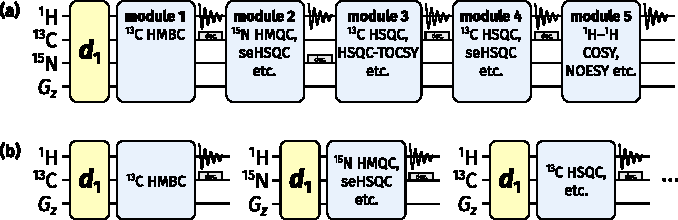
\includegraphics[width=0.8\textwidth]{noah_diagram.pdf}
    {\phantomsubcaption\label{fig:noah_diagram_noah}}
    {\phantomsubcaption\label{fig:noah_diagram_conventional}}
    \caption{
        \textbf{(\subref{fig:noah_diagram_noah})} Diagrammatic representation of a NOAH supersequence, where only one recovery delay (\(d_1\)) is used for the entire experiment.
        \textbf{(\subref{fig:noah_diagram_conventional})} Conventional 2D NMR data acquisition, where one recovery delay is used per dataset.
    }
    \label{fig:noah_diagram}
\end{figure}

Virtually all common 2D experiments employed for small molecule characterisation have been implemented in NOAH supersequences to date, including HMBC, HSQC, HSQC-TOCSY, HMQC, COSY, TOCSY, NOESY, and ROESY.
Each module is given a unique abbreviation, usually one letter long (e.g.\ `B' for HMBC, `S' for HSQC, `M' for HMQC, `C' for COSY) and occasionally sub/superscripted (e.g.\ `S\textsuperscript{T}' for HSQC-TOCSY or `S\textsuperscript{+}' for seHSQC).
The combinatorial nature of NOAH experiments means that there are a very large number of conceivable supersequences ranging from NOAH-2 to NOAH-5 (where the suffix indicates the number of modules); \changed{the use of parallel supersequences\autocite{Kupce2021pNOAH} extends this maximum number even further.}
% In principle, this figure is on the order of \(N^5\), where \(N\) is the number of available modules: as of the time of writing, \(N\) is 27, which in total yields more than 10 million NOAH supersequences.

For optimal data quality in terms of both sensitivity and artefact minimisation, there are certain conditions on NOAH supersequences.
Specifically, NOAH modules placed earlier in a supersequence should ideally utilise only the specific magnetisation they require.
As an example, in the NOAH-2 SC supersequence (HSQC and COSY), the \HC{} HSQC module is designed to excite only the \proton{} nuclei directly attached to the 1.1\%-natural abundance \carbon{} and leave all other proton magnetisation (the ``bulk magnetisation'') along the equilibrium \(+z\) axis.\autocite{SchulzeSunninghausen2014JACS}
A \HH{} COSY module (or TOCSY, or NOESY, etc.) can then draw on this bulk magnetisation, with almost no loss in sensitivity and without having to wait for the \carbon{}-bound protons to relax.
Conversely, if the COSY module were placed first, the \carbon{}-bound proton magnetisation would not survive for use in the HSQC: thus, the HSQC module in a NOAH-2 CS would display severe sensitivity losses, as compared to in a NOAH-2 SC.
More subtle factors also abound, such as in the SBC sequence\autocite{Kupce2017ACIE}, where COSY intensities are modulated by \(T_2\) relaxation and \(J_{\ch{HH}}\) evolution.
The alternative BSC arrangement\autocite{Kupce2018CC}, especially with isotropic ``ASAP'' mixing applied before the COSY, circumvents this issue and has become the preferred implementation for HMBC/HSQC combinations\autocite{Claridge2019MRC}.

Considerations such as these restrict the set of ``viable'' NOAH supersequences.
Even so, the original NOAH paper alone suggests a figure of 285\autocite{Kupce2017ACIE}, and the number of available modules has only grown since then.
By our calculations, as of the time of writing, there are
\(\text{\ee{(\nmoda*\nmodb*\nmodc*\nmodd*\nmode)-1-(\nmoda+\nmodb+\nmodc+\nmodd+\nmode-5)-((\nmoda-1)*(\nmodb-1)*(\nmodc-1)*(\nmodd-1)*\nmoddoublehom)-(\nmode-1)-(\nmoda*\nmodb*\nmoddup*\nmode)+(\nmoddup)}}\)
viable NOAH supersequences (\cref{sec:combinations}).
Constructing every one of these supersequences ``by hand'' is clearly unreasonable.
Consequently, it has not been possible to produce an exhaustive series of pulse programmes: we have so far had to limit ourselves to a handful of ``typical'' supersequences, which may or may not be applicable to all users' needs.

To solve this problem, we sought to \textit{programmatically} generate NOAH pulse programmes, an approach which we term GENESIS (GENEration of Supersequences In Silico).
The implementation of this is a single web page (\cref{fig:screenshot}), accessible via \theurl{}, which can construct virtually any supersequence one might want and output a Bruker pulse programme ready for download and execution.
\changed{
    Apart from allowing users to download customised supersequences, this allows us to easily and rapidly disseminate new NOAH developments to users, independently of TopSpin's own release cycle and without needing a separate publication for each.
    Such developments may include either new modules or updates to existing modules, as detailed later in this article.
    Adopting a programmatic approach also ensures that the output is predictable and can be reasoned about; this eliminates many possibilities of user error during pulse programme construction, a particularly acute problem for NOAH sequences which tend to have considerable length.
}

The regular GENESIS user interface is designed to only produce viable supersequences: thus, for example, it is not possible to create the CS or SBC supersequences discussed earlier.
This is most useful for ordinary users who wish to follow established best practices.
For more advanced usage, enabling ``developer mode'' will remove these limitations, allowing any arbitrary combination of modules to be created.
\changed{
    The website further contains an extensive library of frequently asked questions about the implementation and practical details of NOAH experiments.
    It also offers download links for the AU scripts used for processing, as well as the new Python script used for toggling non-uniform sampling on/off (\texttt{noah\_nus2.py}, discussed in \cref{subsec:nus}).
}

\begin{figure}
    \centering
    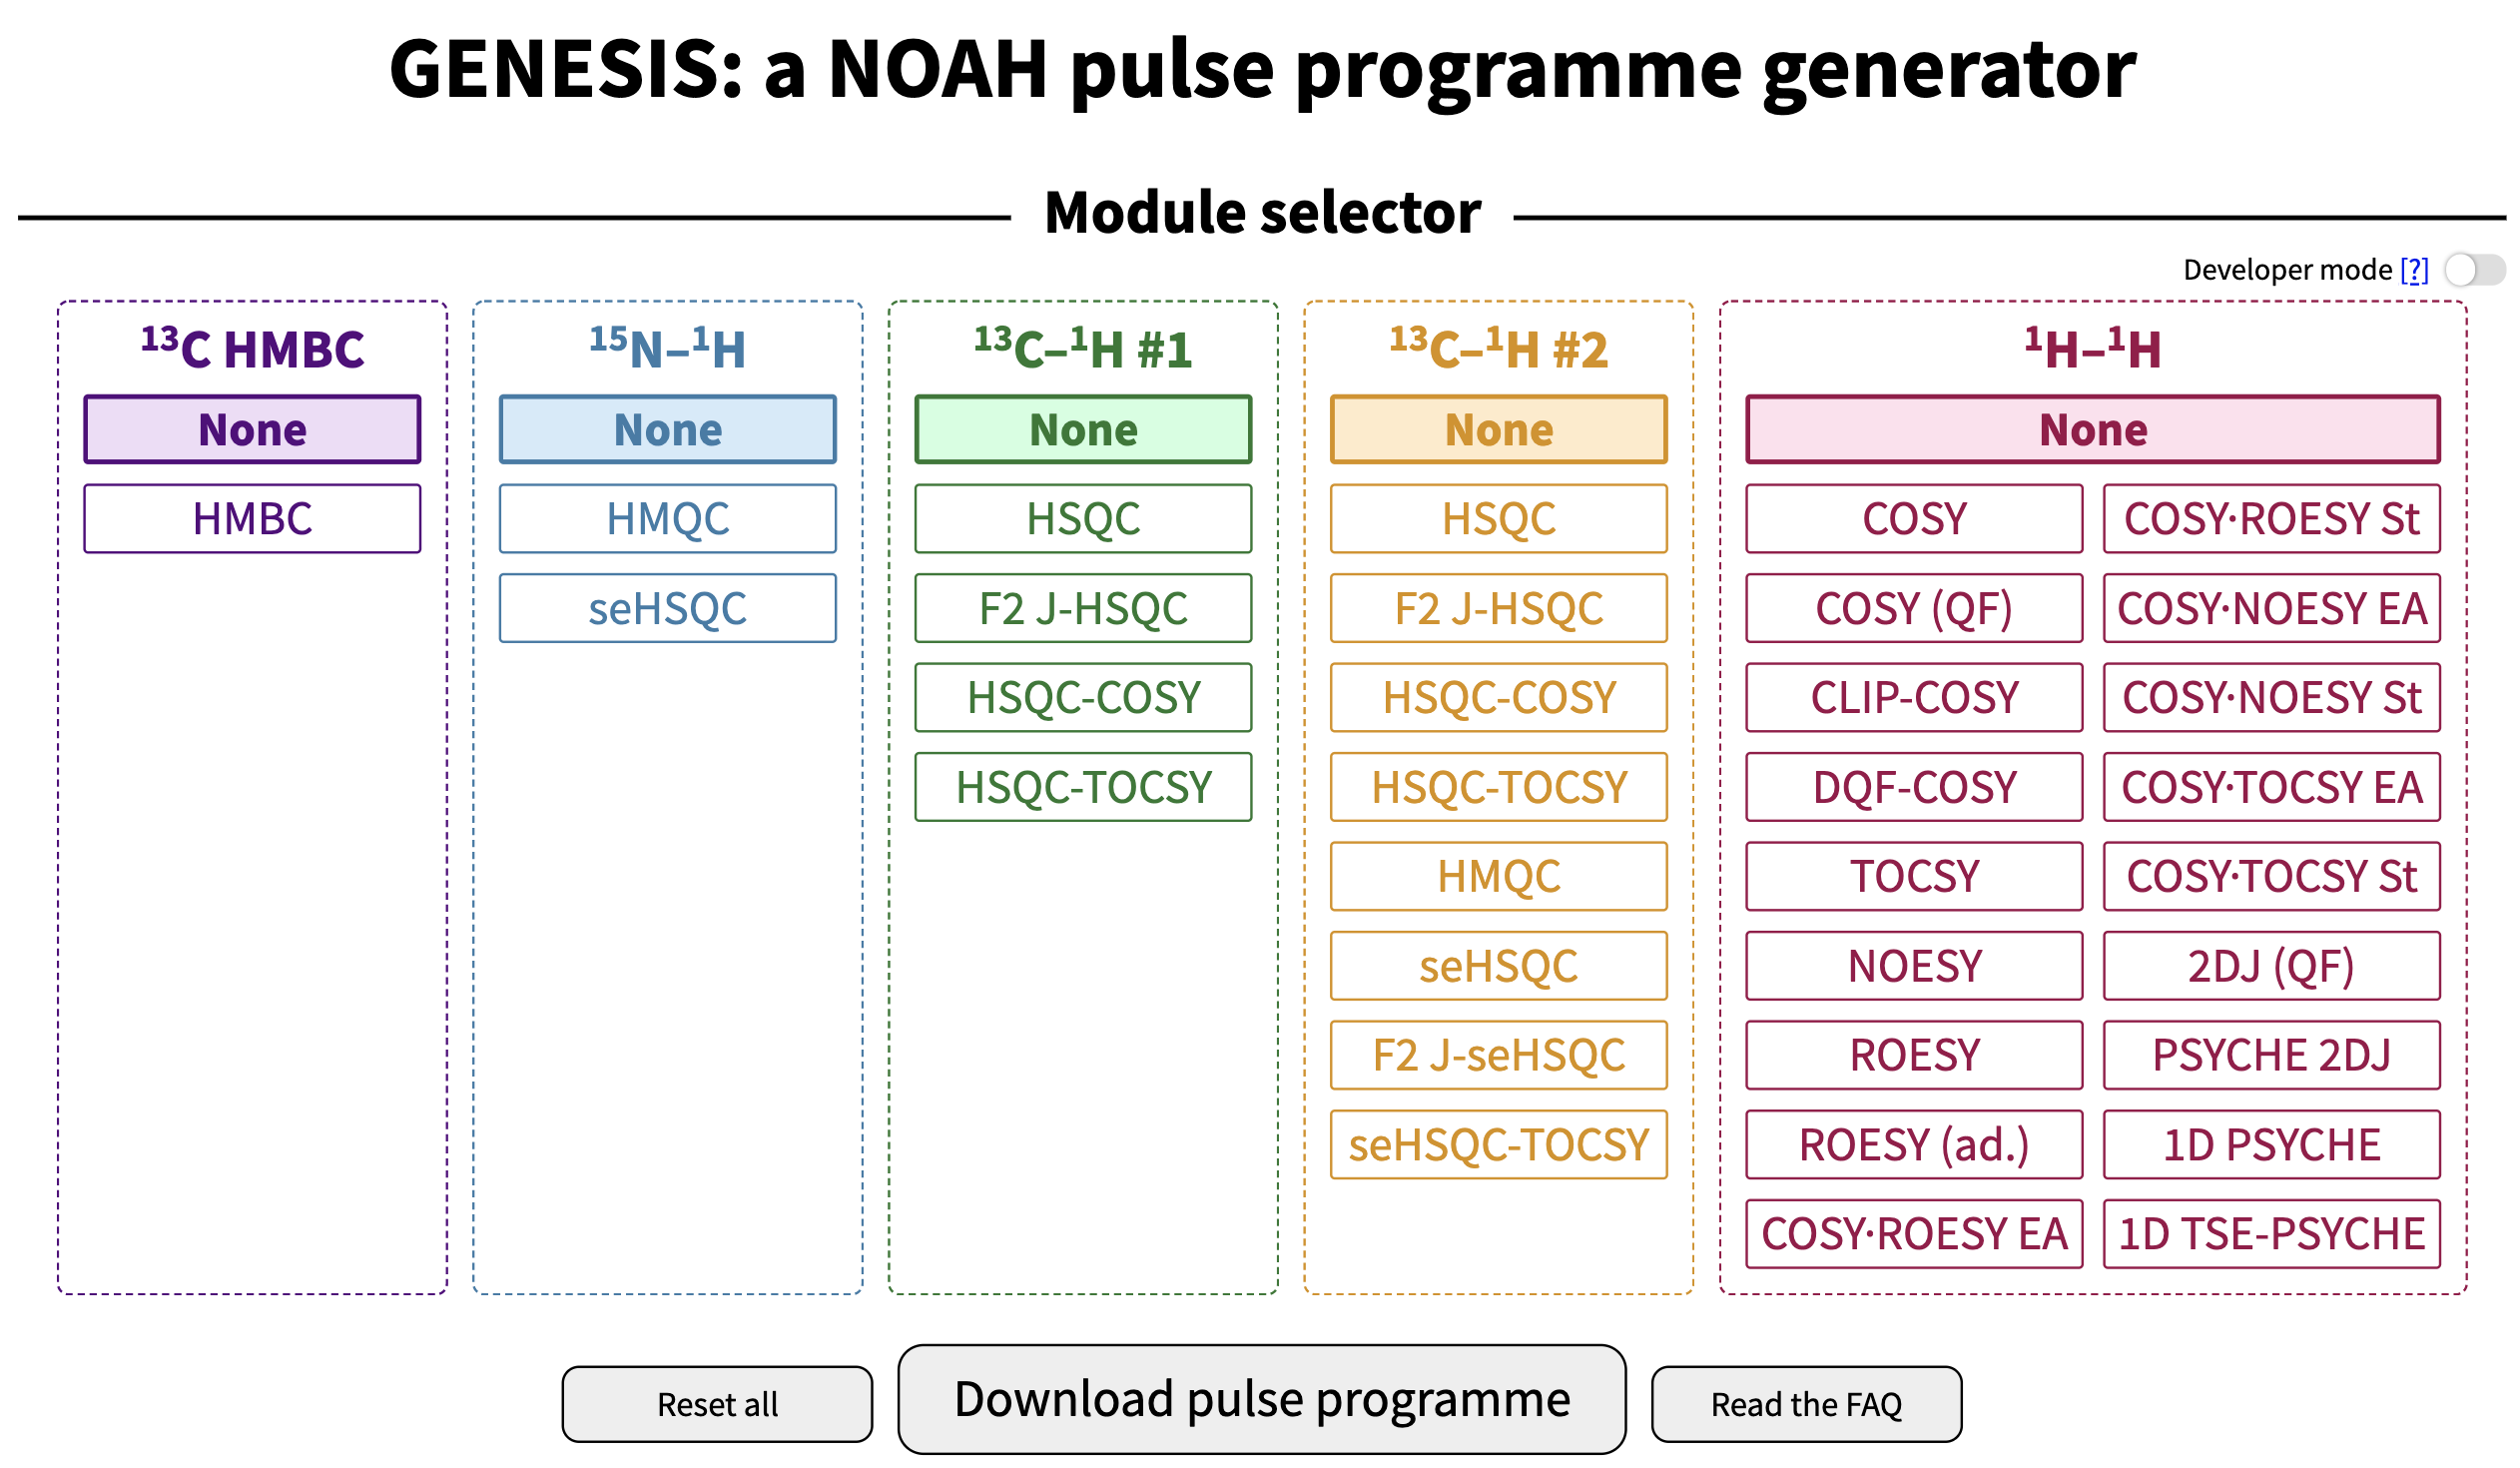
\includegraphics[width=0.8\textwidth]{screenshot.png}
    \caption{
        A screenshot of the GENESIS web interface.
        Visible here are the module choices, the ``developer mode'' toggle, and buttons for downloading the pulse programme.
    }
    \label{fig:screenshot}
\end{figure}

\section{Implementation details}

We begin with a brief discussion of how the GENESIS approach works.
The pulse programme generation code itself is written in TypeScript (version 4.2.3, Microsoft), which is compiled to JavaScript (formally ECMAScript 2015, or ``ES6'') and then executed directly in a client's browser; there is no server-side code.
The web browser shows a list of modules for users to choose from, using accessible and familiar names such as HMBC, HSQC, and so on (\cref{fig:screenshot}).
Internally, these are mapped to a series of \texttt{NOAHModule} objects, each of which contain module-specific information, such as its abbreviation, the requisite parameter definitions, the pulse programme for the module itself, and the appropriate AU programme to be used for processing. 

\begin{figure}
    \centering
    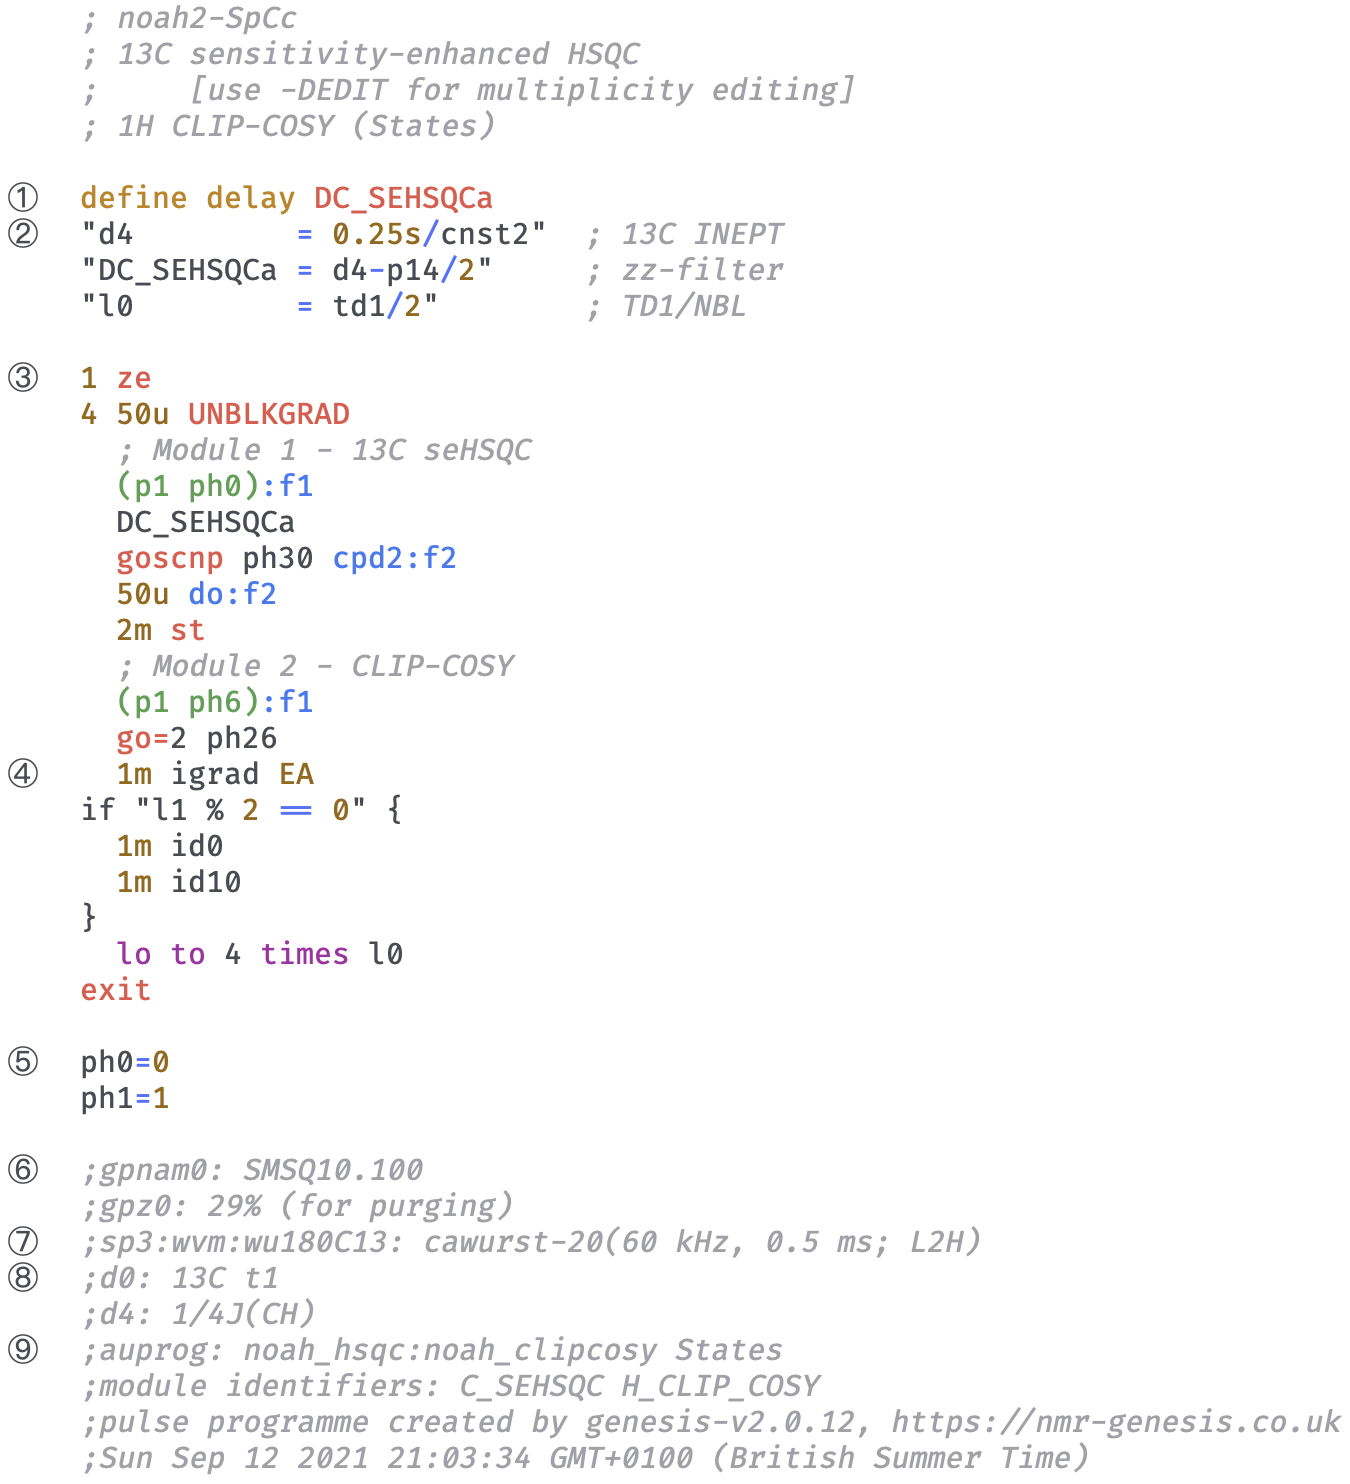
\includegraphics[width=0.8\textwidth]{pulprog_code.png}
    \caption{
        Abridged pulse programme for a NOAH-2 \(\mathrm{S^+C^c}\) supersequence (\carbon{} seHSQC + CLIP-COSY).
        Specific sections of interest are numbered on the left.
        \textbf{(1)} Module-specific delays are given unique identifiers to prevent clashes and to improve readability.
        \textbf{(2)} TopSpin parameters (delays such as \texttt{d4}) are standardised between modules.
        \textbf{(3)} The pulse programme instructions themselves begin here.
        \textbf{(4)} \(t_1\) incrementation and echo--antiecho gradient inversion is carried out \changed{as necessary}.
        \textbf{(5)} Pulse and receiver phase cycles are standardised between modules.
        \textbf{(6)} Comments for gradient pulses are compatible with the TopSpin \texttt{gppp} script.
        \textbf{(7)} Instructions for generating shaped pulses using TopSpin's WaveMaker software.
        \textbf{(8)} Comments describing each parameter appear in the parameter setup screen.
        \textbf{(9)} Instructions for processing AU programmes (\cref{subsec:splitx_au}) are encoded here, along with information about the specific modules used and a timestamp which ensures reproducibility.
    }
    \label{fig:pulprog_code}
\end{figure}

Using this information, GENESIS then constructs the pulse programme in several steps (\cref{fig:pulprog_code}):

\begin{itemize}
    \item Header comments including information about the pulse programme and constituent modules;
    \item Parameter definitions from each module are then collated, taking particular care to avoid duplicate definitions for parameters used in multiple modules;
    \item The main section, which contains the actual instructions for the pulse sequence, is then put together.
        This is done mostly by concatenating individual modules together, although there are also context-sensitive blocks placed \textit{between} modules such as purge pulses, gradients, or ASAP mixing\autocite{Claridge2019MRC} in BSX-type supersequences (X being any homonuclear module);
    \item Appropriate looping and incrementation of parameters such as phase cycles, \(t_1\) delays, and gradient amplitudes for echo--antiecho selection is added at the end of the main section;
    \item Additional comments containing descriptive text for parameters (displayed in TopSpin's \texttt{ased} parameter setup screen), as well as gradient and shaped pulse information (which allow direct setup using the \texttt{gppp} and \texttt{wvm} commands), are added at this stage.
        These are collated by scanning the main section for TopSpin parameters (e.g.\ delays, pulses, gradients) and obtaining their descriptions from a lookup table;
    \item Finally, we also specify the exact modules used in the pulse programme, the GENESIS version number, and a timestamp. \changed{This is important for reproducibility purposes (\cref{subsec:repro}).}
\end{itemize}


\subsection{Standardisation of parameter meanings}

An immediate problem of directly concatenating pulse programme texts from different modules is that a given parameter in one module may take on a different meaning in another module.
As a necessary step to prevent such clashes, we have fully standardised all parameters used in the GENESIS pulse programmes.
These include pulse widths (\texttt{p}), delays (\texttt{d}), constants (\texttt{cnst}), \(z\)-gradient amplitudes (\texttt{gpz}), and phase cycles (\texttt{ph}).
Where possible, we have chosen meanings that are similar to those in the standard library of Bruker pulse programmes, \changed{only deviating in order to avoid inevitable clashes between different modules.}
% However, there are invariably some small deviations: for example, the \(\Delta'\) delay in both the \HC{} and \HN{} sensitivity-enhanced HSQC sequences (which can range from \(1/(8 \cdot\onejxh)\) to \(1/(4 \cdot\onejxh)\))\autocite{Schleucher1994JBNMR} is referred to as \texttt{d24} in the standard library.
% \changed{To avoid a clash in NOAH supersequences involving both seHSQC modules,\autocite{Yong2021JMR} we have to assign these to different delays.}
Furthermore, in place of module-specific delays which are often called \texttt{DELTA1}, \ldots{} in standard library sequences, we have chosen to define new identifiers with more human-readable names inside the pulse programme itself.
Thus, the delays in a HSQC sequence might be called \texttt{DC\_HSQC1}, \ldots{}, where the first \texttt{C} indicates the indirect-dimension nucleus (\carbon{}).

While this standardisation was primarily implemented in order to facilitate pulse programme construction, this also makes it far easier for users to set up NOAH experiments.
\changed{
    Since the majority of these parameters are consistent with the standard library, many of them may be directly read in from the \textit{prosol} relation tables and/or existing parameter sets in TopSpin.
    Furthermore, since every parameter has the same meaning in every NOAH supersequence, it also makes setting up multiple supersequences an almost trivial task: generally only the parameters \texttt{NBL}, \texttt{PULPROG}, and \texttt{TD1} need be changed.
}

\subsection{Choice of module versions}

\begin{figure}[ht]
    \centering
    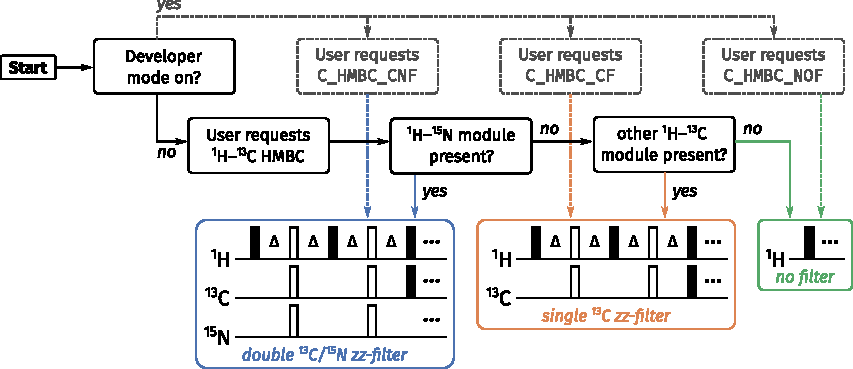
\includegraphics[width=0.85\textwidth]{flowchart.pdf}
    \caption{
        Flowchart illustrating how GENESIS decides the form of the \(zz\)-filter to be used in a \HC{} HMBC module.
        Dotted lines represent the branch where developer mode is enabled, i.e.\ the user has full control over which form is used: these are labelled by alphabetical codes starting with \texttt{C\_HMBC} (the website contains a full description of these codes).
        Solid lines represent the standard user mode, i.e.\ developer mode disbaled: in this case, GENESIS automatically chooses the appropriate module based on what other modules are present in the supersequence.
    }
    \label{fig:flowchart}
\end{figure}

Another potential issue is that different versions of a pulse sequence often exist.
An example is the \(zz\)-HMBC, where the \(zz\)-filter element is used to retain \carbon{}-bound and/or \nitrogen{}-bound \proton{} magnetisation.\autocite{Kupce2018CC,Kupce2019JMR}
Since the user only specifies that they want a HMBC module and not the exact details of the \(zz\)-filter, the GENESIS code must in effect make this choice for the user behind the scenes, \changed{in an adaptive fashion which changes depending on what other modules the user selects (\cref{fig:flowchart}).
Advanced users may, however, circumvent this and make their own choice by entering ``developer mode'': each version is assigned a different label \texttt{C\_HMBC\_...} (the labels are enumerated in more detail on the website).
}
The sensitivity-enhanced HSQC (seHSQC, abbreviated `\(\mathrm{S^+}\)'/\texttt{Sp}) presents a similar case.
If the seHSQC module is followed by one or more homonuclear modules such as a COSY or NOESY, then the ZIP-seHSQC\autocite{Hansen2021AC,Yong2021JMR} is automatically chosen, as this preserves the requisite magnetisation for the later modules.
However, if the seHSQC module is used last in the sequence, then the original Cavanagh--Rance--Kay seHSQC\autociteset{sehsqc} is chosen in order to maximise sensitivity.


\subsection{Reproducibility}
\label{subsec:repro}

\changed{
    Reproducibility is a key consideration for scientific code, including GENESIS.\autocite{Perkel2020N}
    The primary aim of GENESIS is to release updates to NOAH supersequences in a timely fashion.
    However, it is also important that old releases of pulse sequences remain available so that scientific results using these pulse sequences may be reproduced. 
    Furthermore, each release is accompanied by a suite of processing scripts; these may also be modified over time, and to ensure compatibility with the pulse sequences, old versions of the scripts must also be kept available.
}

\changed{
    To ensure that NMR experiments run with GENESIS pulse programmes and scripts are always reproducible, each pulse programme and script is marked with a version number (labelled \textbf{(9)} in \cref{fig:pulprog_code}).
    Old versions of GENESIS may be obtained using the following formula: to access version \texttt{vX.Y.Z} (where \texttt{X}, \texttt{Y}, \texttt{Z} are integers), navigate to the URL \texttt{https://nmr-genesis.co.uk/X/Y/Z}.
    For example, the release version that accompanies this paper is labelled \texttt{v2.1.0}; this can be accessed at \url{https://nmr-genesis.co.uk/2/1/0}.
    While earlier versions are also available, these should be considered to be ``in-development'' versions, to be used at the reader's own risk.
    As an alternative, the GENESIS code can be obtained from GitHub at \url{https://github.com/yongrenjie/genesis}. Instructions on how to use this are provided in the repository description.
}


\section{Other NOAH improvements within GENESIS}

\changed{
    We now detail a few recent improvements to NOAH supersequences, which are already implemented in the live GENESIS webpage.
    It is worth noting that because of the modular nature of pulse programme construction, changing the underlying code for a single NOAH module is sufficient to propagate changes to all supersequences containing that module.
}

\subsection{Suppression of one-bond artefacts in HMBC}

\begin{figure}[ht]
    \centering
    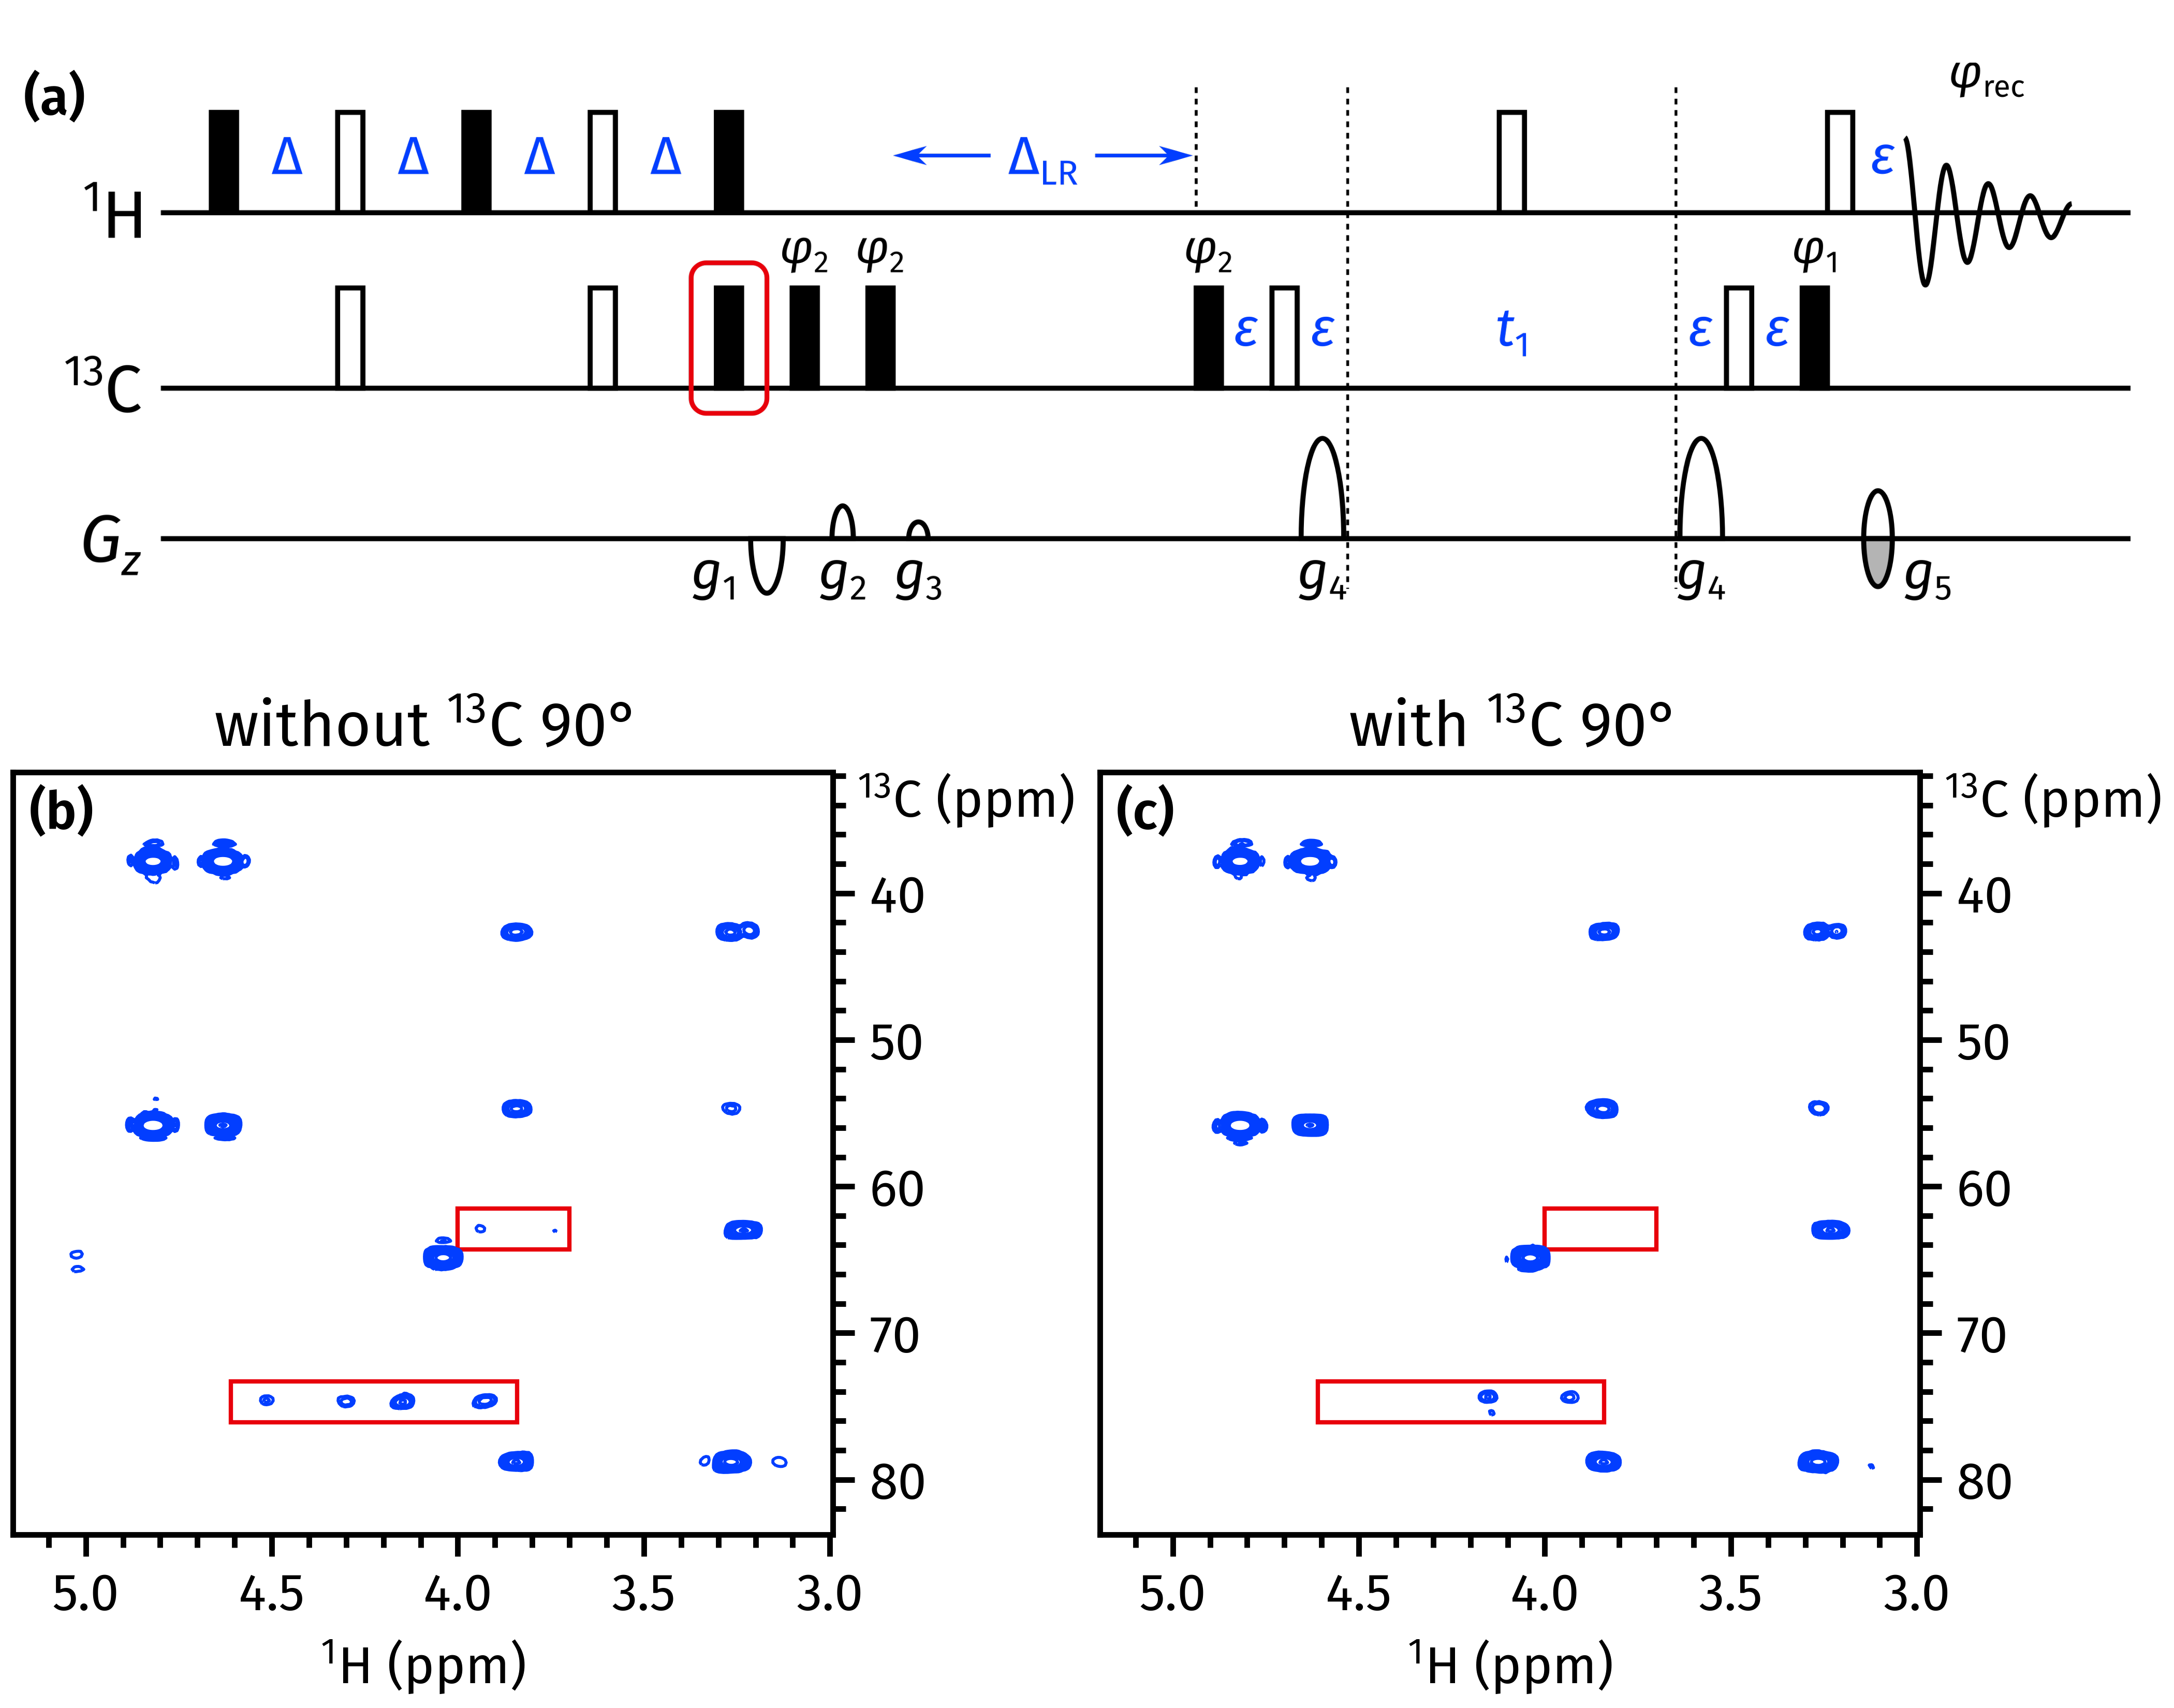
\includegraphics[width=0.7\textwidth]{hmbc_comp.png}
    {\phantomsubcaption\label{fig:hmbc_comp_pulprog}}
    {\phantomsubcaption\label{fig:hmbc_comp_before}}
    {\phantomsubcaption\label{fig:hmbc_comp_after}}
    \caption{
        \textbf{(\subref{fig:hmbc_comp_pulprog})} The NOAH \(zz\)-HMBC pulse sequence, with the newly added \carbon{} \ang{90} pulse highlighted in red.
        The delays are \(\Delta = 1/(4 \cdot \onejch)\) and \(\Delta_{\text{LR}} = 1/(2 \cdot \njch)\); \(\varepsilon\) is the minimum time required for a gradient plus the subsequent recovery delay.
        Phase cycling is performed as follows: \(\phi_1 = x, -x\); \(\phi_2 = x, x, -x, -x\); \(\phi_{\text{rec}} = x, -x, -x, x\).
        All gradients have duration \SI{1}{ms}; amplitudes as a fraction of the maximum gradient strength (\SI{55.7}{G\per\cm}) are as follows: \(g_1 = -15\%\); \(g_2 = 10\%\); \(g_3 = 5\%\); \(g_4 = 80\%\); \(g_5 = \pm 40.2\%\).
        \textbf{(\subref{fig:hmbc_comp_before})} HMBC spectrum obtained using the original \(zz\)-HMBC module, i.e.\ without the added \ang{90} pulse.
        \(\onejch{}\) artefacts are highlighted in red boxes.
        \textbf{(\subref{fig:hmbc_comp_after})} HMBC spectrum obtained with the added \ang{90} pulse.
        \andro{}
    }
    \label{fig:hmbc_comp}
\end{figure}

The \(zz\)-HMBC module is ordinarily placed first in a supersequence, where the \(zz\)-filter element serves to preserve magnetisation of protons directly coupled to \carbon{} and/or \nitrogen{}.\autocite{Kupce2018CC,Kupce2019JMR}
Specifically, the \(zz\)-filter acts as a \ang{90} excitation pulse on uncoupled protons, while leaving coupled protons along \(+z\).
This is largely accomplished in practice, as evidenced by the fact that the intensities in subsequent HSQC-type modules are barely perturbed.
However, not all of the coupled magnetisation is perfectly retained: in particular, the \(zz\)-filter also generates a degree of \textit{antiphase} \(\onejch{}\) magnetisation of the form \(2\mathrm{H}_x\mathrm{C}_z\).
This antiphase magnetisation is later refocused during the low-pass J-filter (LPJF) to give in-phase magnetisation, eventually ending up as one-bond correlation artefacts in the HMBC spectrum (\cref{fig:hmbc_comp_before}).

A simple solution to this is to add a \carbon{} \ang{90} pulse at the end of the \(zz\)-filter (\cref{fig:hmbc_comp_pulprog}): this converts any antiphase magnetisation to double- or zero-quantum magnetisation, which is \changed{subsequently dephased} by the LPJF.
This idea has previously been used by Luy and coworkers in CLIP-HSQC experiments to remove antiphase contributions prior to FID detection.\autocite{Enthart2008JMR}
In the event, this small modification proved to have a large impact, almost completely suppressing the \(\onejch\) artefacts (\cref{fig:hmbc_comp_after}).
Further comparisons of artefact intensity are provided in \cref{sec:si_hmbc}.

\subsection{\texorpdfstring{\nitrogen{}}{15N} HMQC gradient scheme}

\begin{figure}[ht]
    \centering
    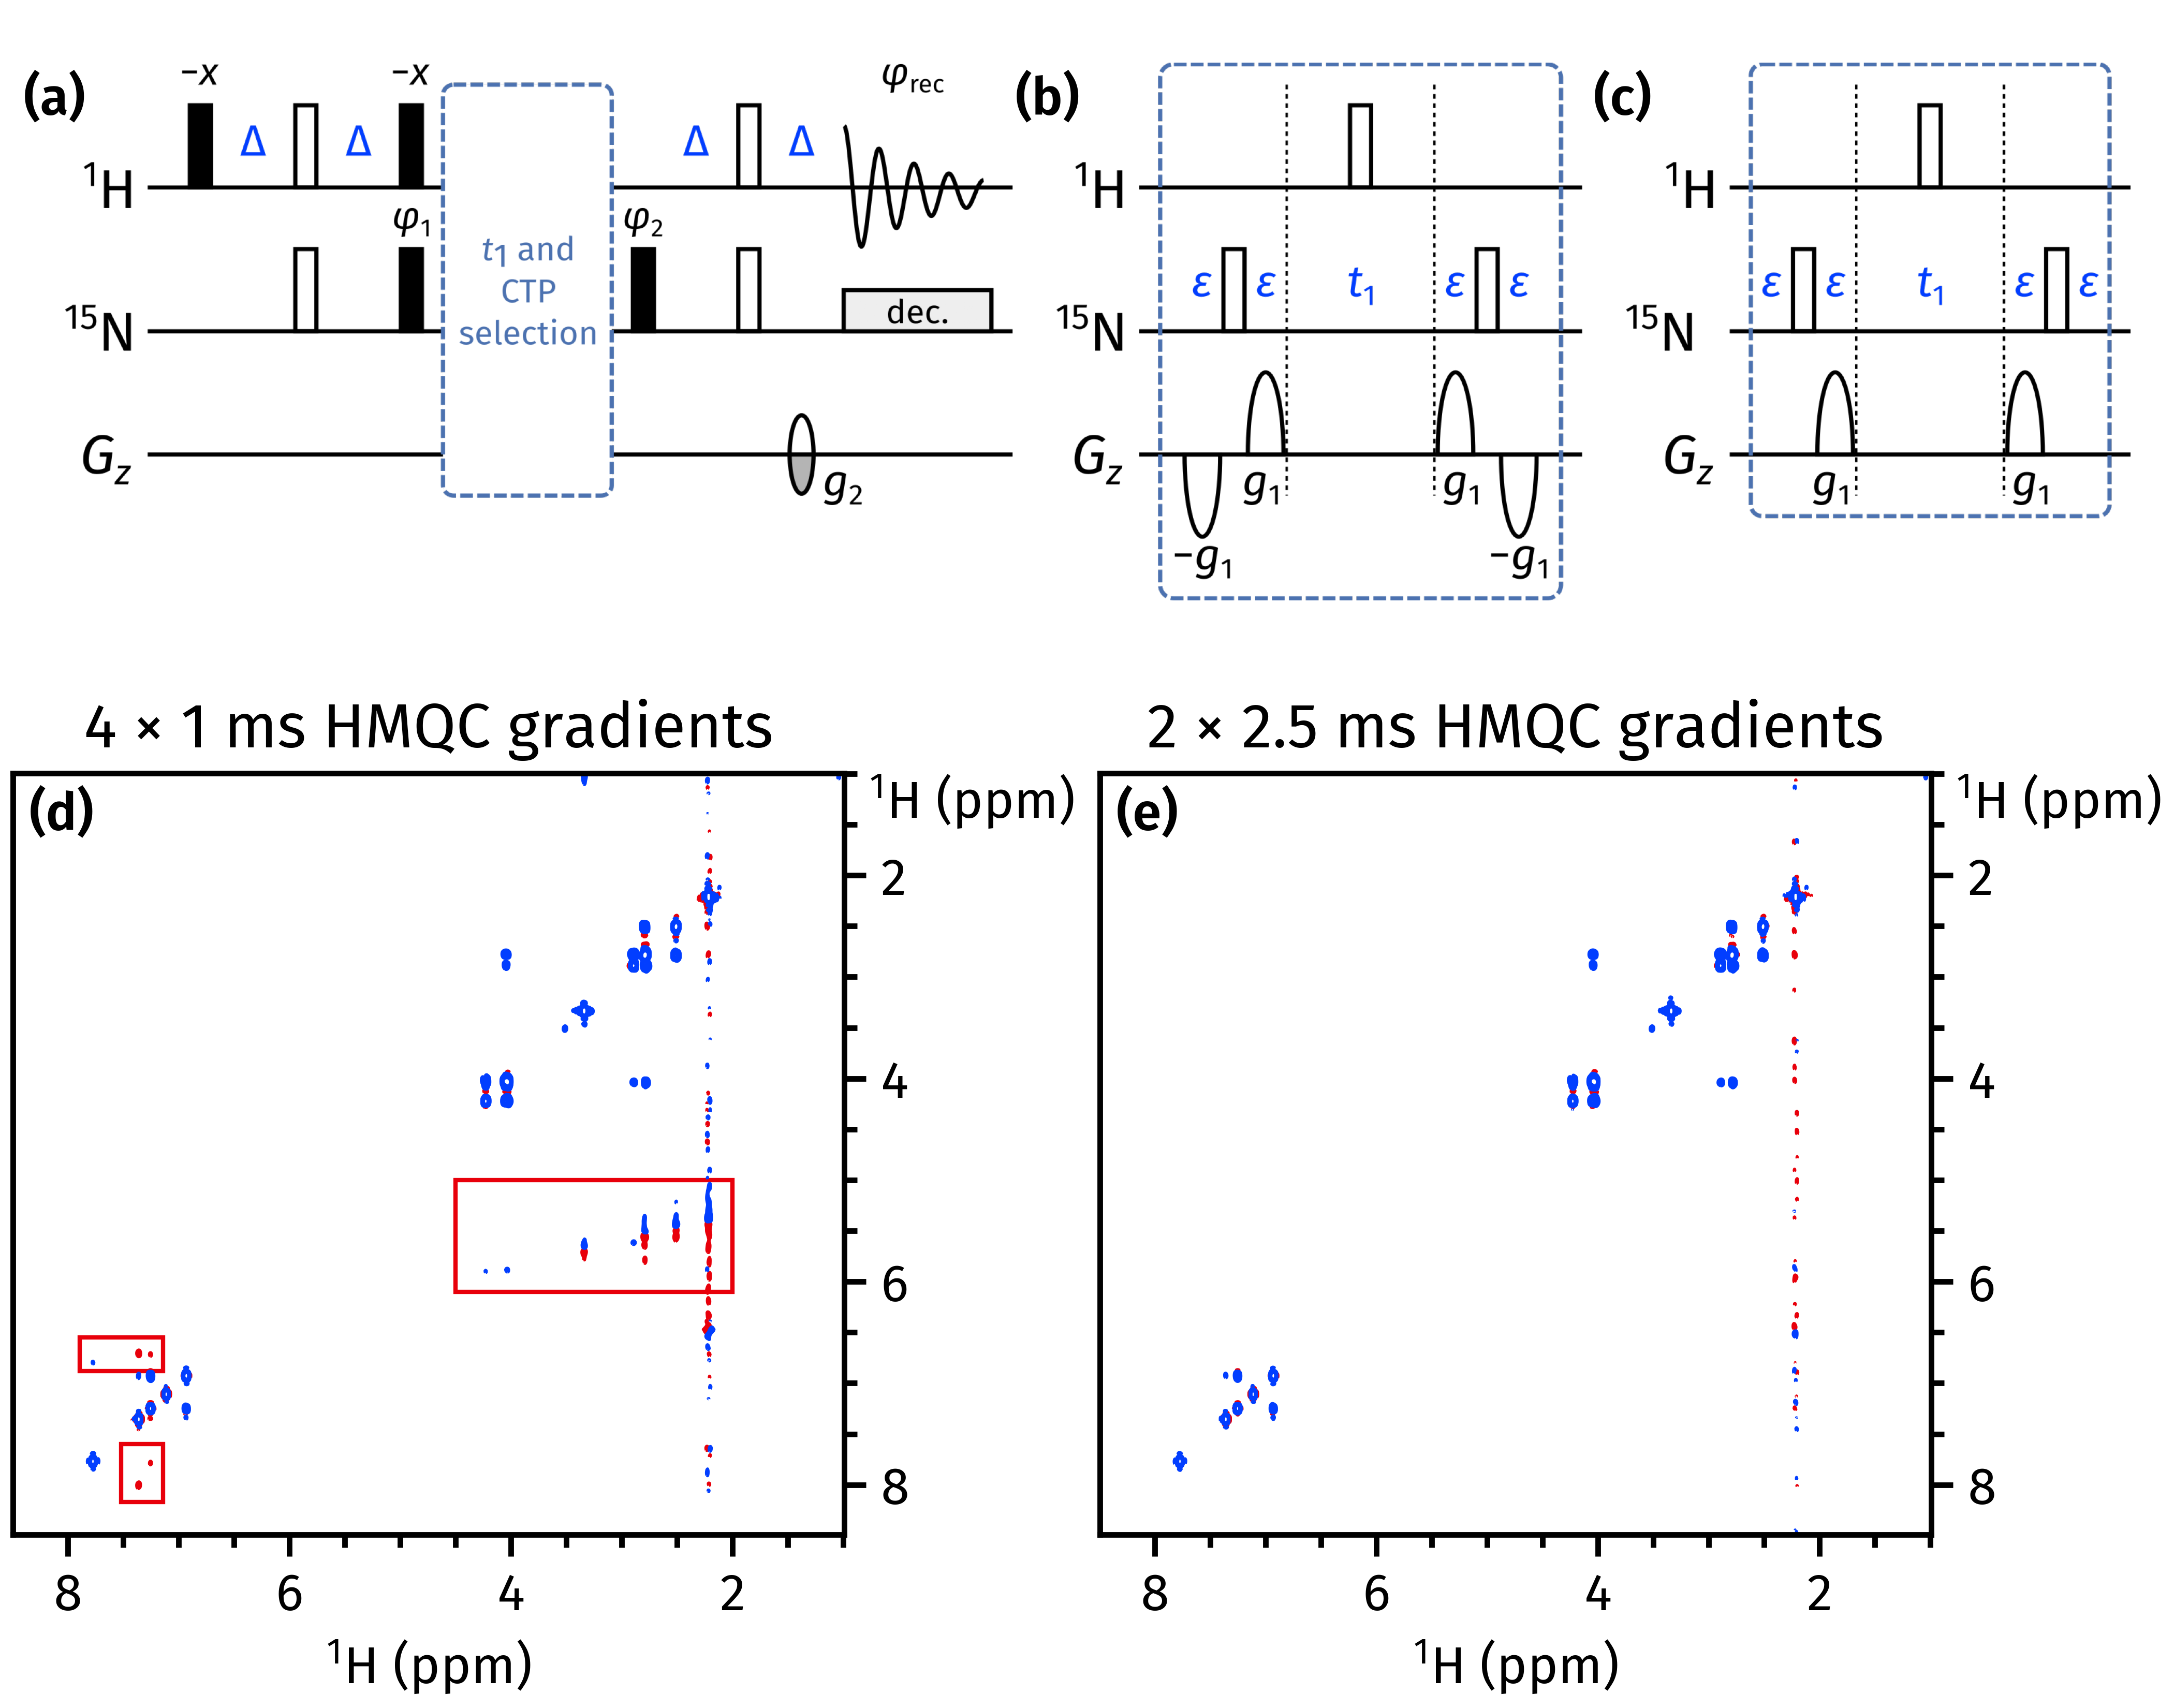
\includegraphics[width=0.7\textwidth]{hmqc_comp.png}
    {\phantomsubcaption\label{fig:hmqc_comp_pulprog}}
    {\phantomsubcaption\label{fig:hmqc_comp_pulprog_before}}
    {\phantomsubcaption\label{fig:hmqc_comp_pulprog_after}}
    {\phantomsubcaption\label{fig:hmqc_comp_spec_before}}
    {\phantomsubcaption\label{fig:hmqc_comp_spec_after}}
    \caption{
        \textbf{(\subref{fig:hmqc_comp_pulprog})} A general outline of the NOAH \nitrogen{} HMQC module.
        \(g_2\) has a duration which matches that of \(g_1\) (explained below), and an amplitude of \(\pm n \cdot 8.1\%\), where \(n\) is the number of CTP gradients bracketing the \(t_1\) period.
        \(g_1\) has an amplitude of \(80\%\) in all cases.
        All other symbols have the same meaning as in \cref{fig:hmbc_comp}.
        \textbf{(\subref{fig:hmqc_comp_pulprog_before})} The previously published coherence selection scheme for the HMQC module, with four gradients each of duration \SI{1}{ms}.
        \textbf{(\subref{fig:hmqc_comp_pulprog_after})} The new coherence selection scheme for the HMQC module, with two gradients each of duration \SI{2.5}{ms}.
        \textbf{(\subref{fig:hmqc_comp_spec_before})--(\subref{fig:hmqc_comp_spec_after})} CLIP-COSY spectra obtained from a NOAH-3 \(\mathrm{MS^+C^c}\) supersequence (\nitrogen{} HMQC + \carbon{} seHSQC + CLIP-COSY), acquired with the gradient schemes shown in (\subref{fig:hmqc_comp_pulprog_before}) and (\subref{fig:hmqc_comp_pulprog_after}) respectively.
        The wing artefacts in the former spectrum are highlighted in red boxes.
        \zolmi{}
    }
    \label{fig:hmqc_comp}
\end{figure}

We have recently described the occurrence of ``wing artefacts'' in homonuclear modules, which arise from bulk magnetisation which evolves during either half of \(t_1\) in a preceding heteronuclear module.\autocite{Yong2021JMR}
These artefacts can be removed in an elegant manner by ensuring that each half of \(t_1\) in a HMQC/HSQC/seHSQC module contains coherence transfer pathway (CTP) gradients of equal sign and magnitude, which makes sure that any bulk magnetisation undergoing net evolution during \(t_1\) is dephased.

At the same time, it is also important that the final gradient in the heteronuclear module have as large an amplitude as possible, since this gradient is responsible for dephasing bulk magnetisation that is not returned to \(+z\) just prior to the detection period.
In order to accomplish this, the previous \nitrogen{} HMQC module used bipolar opposing gradients in either half of \(t_1\), a scheme which allows the final refocusing CTP gradient \(g_2\) to have an amplitude of \(4g_1(\gamma_{\ch{N}} / \gamma_{\ch{H}})\) (\cref{fig:hmqc_comp_pulprog_before}).
Although this leads to excellent artefact suppresion in the \nitrogen{} HMQC itself, wing artefacts are apparent in downstream modules (\cref{fig:hmqc_comp_spec_before}), because the opposing gradients cancel each other out and do not enforce any CTP selection on the bulk magnetisation.

The solution to this is to only use two gradients during \(t_1\) (one in either half), and to \textit{lengthen} their duration such that the final gradient \(g_2\) provides sufficient dephasing in the HMQC itself (\cref{fig:hmqc_comp_pulprog_after}).
This strategy was previously described for the \nitrogen{} seHSQC;\autocite{Yong2021JMR} here we have also applied it to the HMQC with success (\cref{fig:hmqc_comp_spec_after}).
This change causes no significant difference in the sensitivity of the HMQC module itself (\cref{fig:hmqc_comp_snr}).

\subsection{PSYCHE and 2DJ modules}

In previous work,\autocite{Yong2021JMR} we described how \HN{} modules could be implemented with optional ``\(k\)-scaling''.\autocite{PerezTrujillo2007MRC}
This entails a reduction in the number of \(t_1\) increments (by a factor of \(k\)), in return for a corresponding increase in the number of transients per increment, with no overall change in the experimental time.
Particularly for the HMQC experiment, this allowed modest gains in sensitivity as \(J_{\ch{HH}}\) splittings were no longer resolved in the indirect dimension.

\begin{figure}[ht]
    \centering
    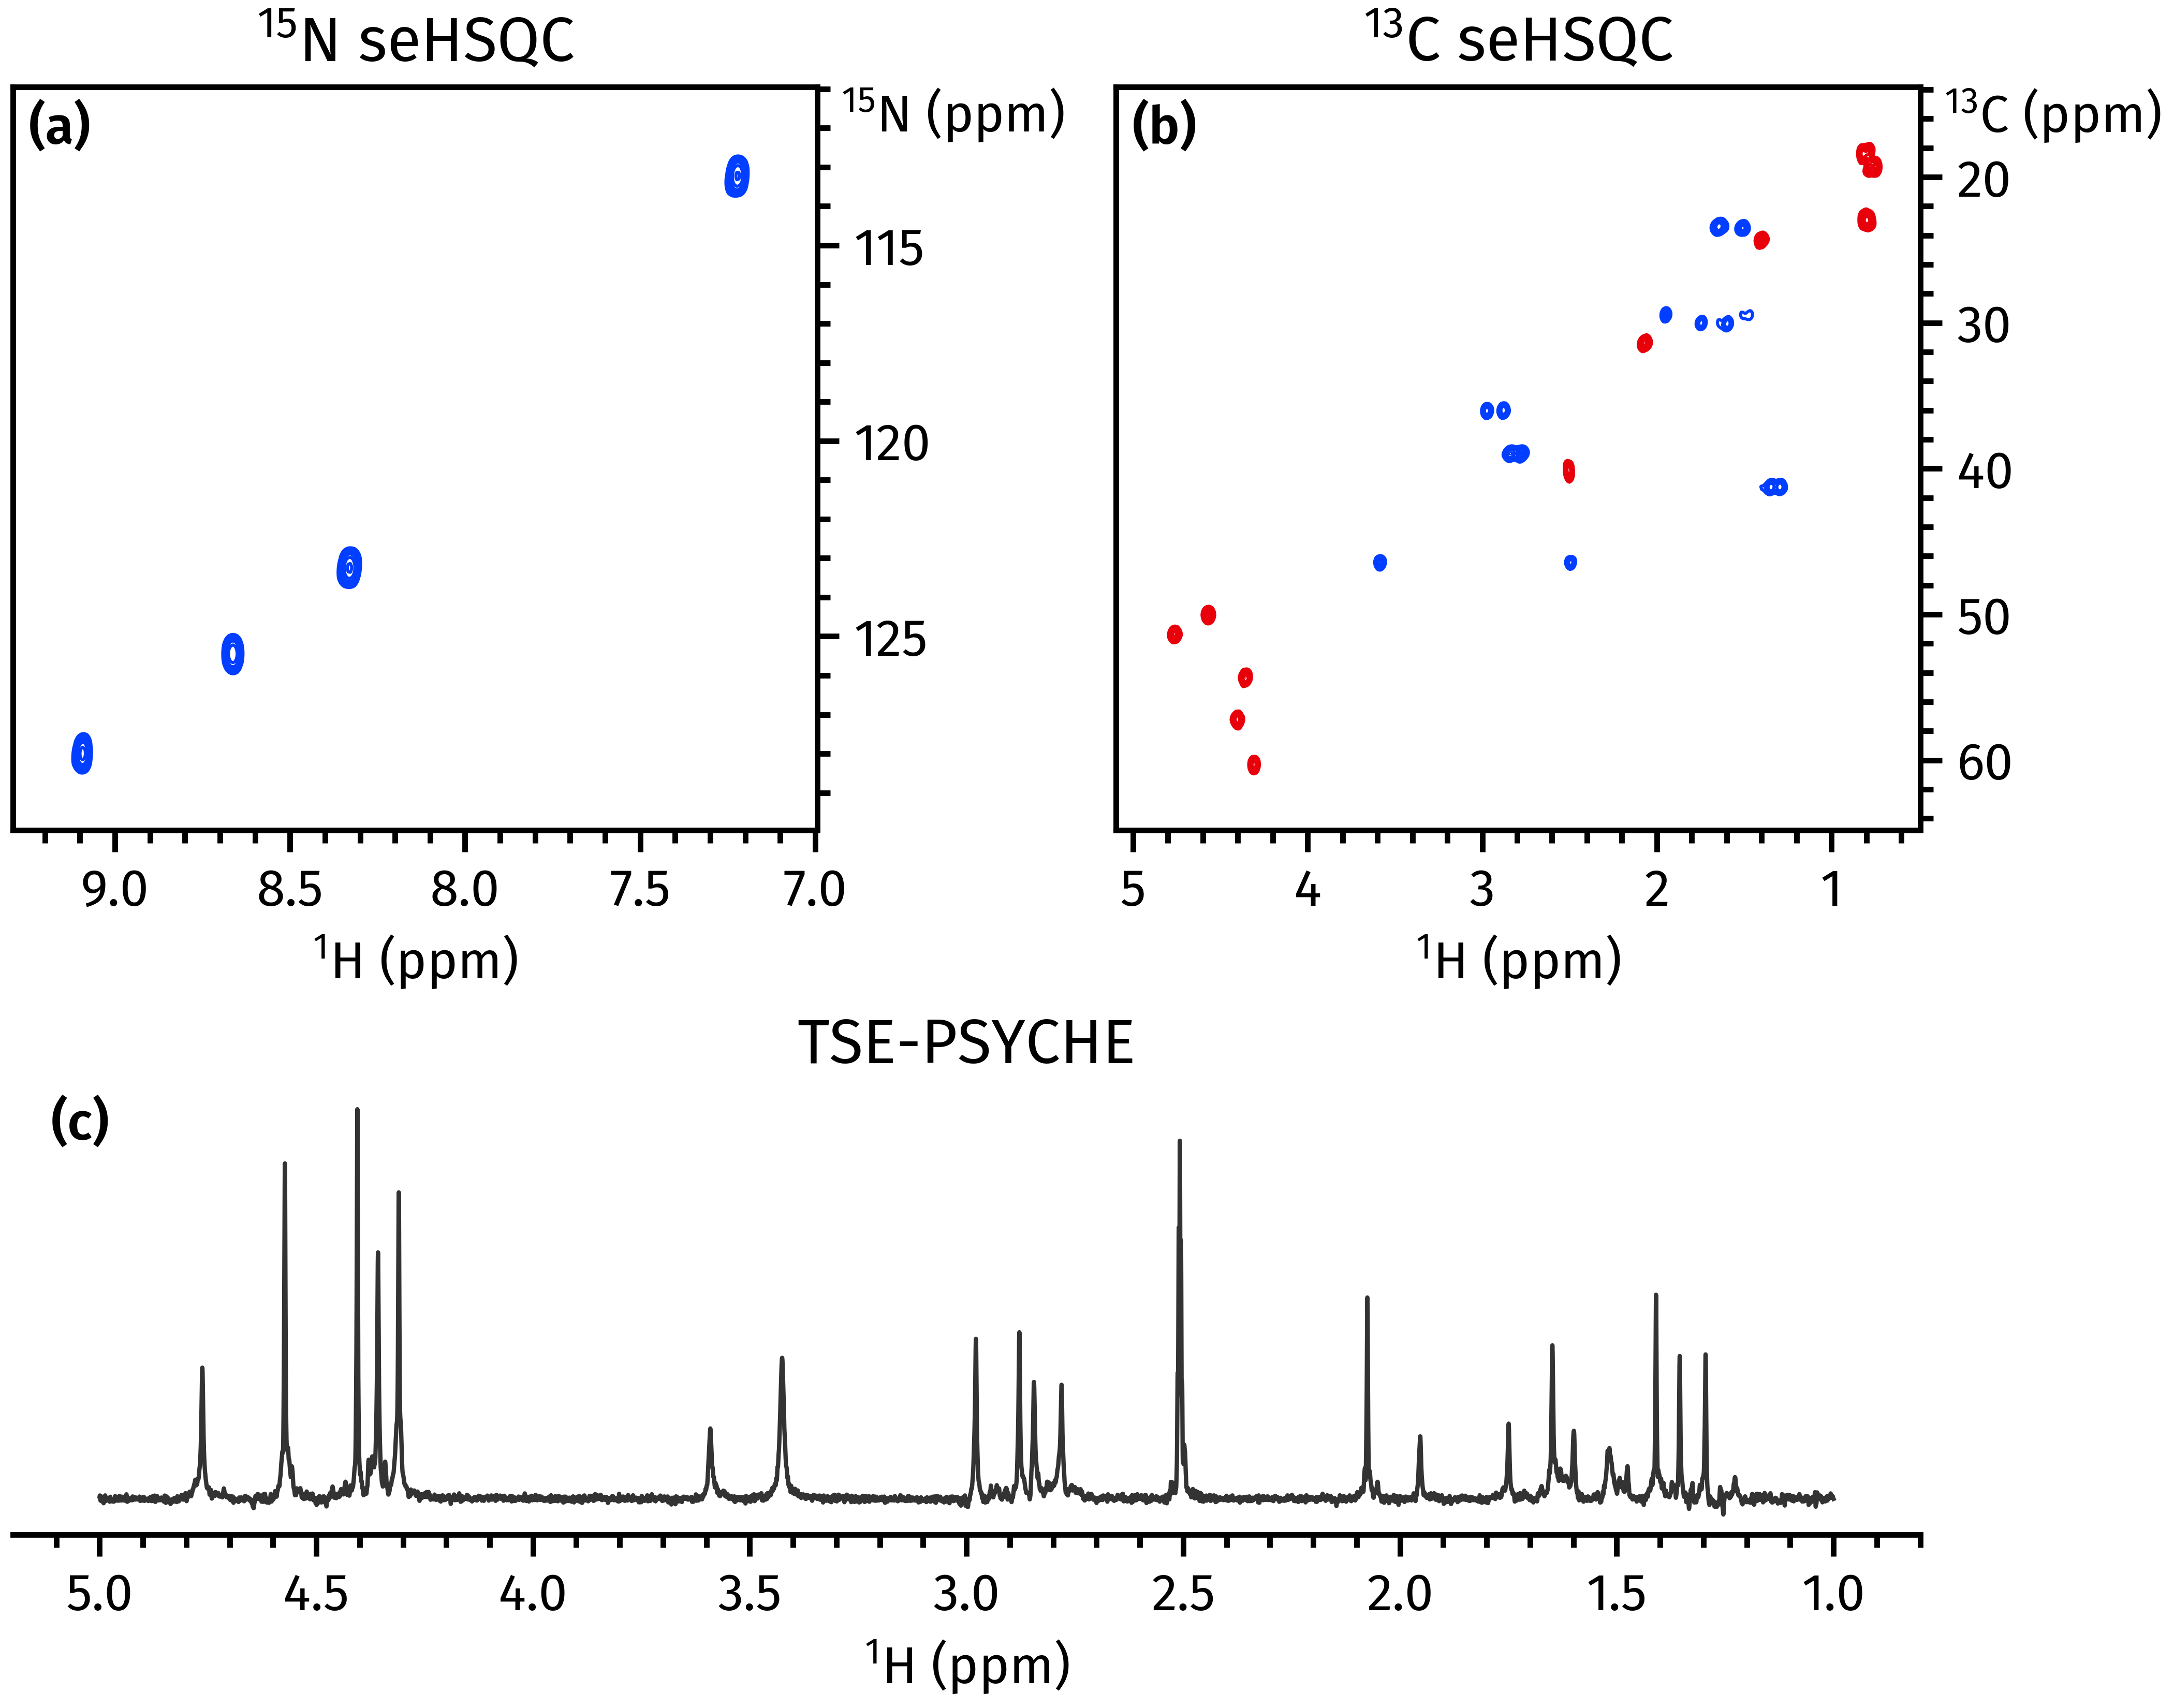
\includegraphics[width=0.7\textwidth]{psyche.png}
    {\phantomsubcaption\label{fig:psyche_n15_sehsqc}}
    {\phantomsubcaption\label{fig:psyche_c13_sehsqc}}
    {\phantomsubcaption\label{fig:psyche_psyche}}
    \caption{
        Spectra obtained from a NOAH-3 \(\mathrm{S^{+}_{N}S^{+}P^T}\) supersequence.
        \textbf{(\subref{fig:psyche_n15_sehsqc})} \nitrogen{} sensitivity-enhanced HSQC\autocite{Yong2021JMR} (256 \(t_1\) increments, 2 scans per increment).
        \textbf{(\subref{fig:psyche_c13_sehsqc})} \carbon{} sensitivity-enhanced HSQC\autocite{Hansen2021AC,Yong2021JMR} (256 \(t_1\) increments, 2 scans per increment).
        \textbf{(\subref{fig:psyche_psyche})} 1D TSE-PSYCHE pure shift spectrum\autocite{Foroozandeh2015CC} (saltire flip angle of \ang{10}, 32 chunks, 16 scans per chunk).
        \grami{}
    }
    \label{fig:psyche}
\end{figure}

A simple extension of this protocol to \textit{homonuclear} \proton{}--\proton{} modules enables experiments such as 2D J-resolved or pseudo-2D pure shift spectroscopy to be incorporated into NOAH supersequences.
In both cases, the number of \(t_1\) increments needed (16--32) is far smaller than the typical number required for a 2D experiment (128--256).
In particular, at present, we have implemented a family of PSYCHE experiments, namely: the original pseudo-2D PSYCHE (abbreviated ``P''); the triple spin echo (TSE)-PSYCHE experiment (``P\textsuperscript{T}''), which provides improved robustness towards strong coupling; and the PSYCHE 2DJ experiment (``J'') which yields pure absorption-mode lineshapes.\autociteset{psyche}
\changed{On top of this, there is also a magnitude-mode 2D J module available (``J\textsuperscript{qf}'').}

In PSYCHE spectra, the flip angle of the chirp or saltire pulses used in the J-refocusing element provides the experimentalist with a choice: a larger flip angle provides greater sensitivity, but at the cost of increased artefacts.\autocite{Foroozandeh2018CEJ}
One advantage of acquiring PSYCHE spectra in NOAH-type supersequences is that, due to the increased number of transients, sensitivity is often not at a premium.
Thus, the user can choose a smaller flip angle (ca.\ \ang{10}) in order to maximise spectral purity instead, without losing any actual spectrometer time.
An example of a NOAH-3 supersequence with the TSE-PSYCHE module is shown in \cref{fig:psyche}.

\subsection{splitx\_au processing}
\label{subsec:splitx_au}

NOAH data processing is done using the \texttt{splitx\_au} AU programme; this is responsible for creating separate datasets containing the data for each module, defining any required processing parameters, and processing each dataset using module-specific AU programmes (e.g.\ \texttt{noah\_hsqc} for \carbon{} HSQC data).
Previously, the names of the module-specific AU programmes had to be specified as the \texttt{USERP1}, \texttt{USERP2}, \ldots{} series of processing parameters.
In contrast, with GENESIS pulse programmes, this information is directly embedded within the pulse programme itself; consequently, with a small modification to the \texttt{splitx\_au} AU programme, we can parse the pulse programme to obtain the requisite list of AU programmes.
The user therefore does not have to specify it explicitly, which makes setting up multiple different supersequences a much smoother process.
If necessary, it is possible to override these ``default'' AU programmes by explicitly specifying the \texttt{USERPn} parameters, allowing for customised processing.

\subsection{Non-uniform sampling implementation}
\label{subsec:nus}

With the GENESIS pulse programmes we also introduce a new and more user-friendly implementation of non-uniform sampling (NUS).
NOAH experiments do not work ``out of the box'' with TopSpin's conventional NUS setup routine: some special adjustments have to be made by manually generating the list of increments to be sampled and adjusting the \(t_1\) delays accordingly within the pulse sequence looping.
Previously, this was accomplished using a Python script which created a new pulse programme for each supersequence, e.g.\ \texttt{noah3\_BSC.nus}.\autocite{Claridge2019MRC}
We have modified this approach such that the \textit{same} pulse programme can be used for both uniform and non-uniform sampling, where NUS is controlled by an acquisition flag \texttt{-DNUS}.
Although a (different) Python script is still required for initialisation, this means that it is no longer necessary to keep two separate instances of the same pulse sequence in TopSpin, and reduces the difficulty of turning NUS on and off.


\section{Conclusion}

Here, we have demonstrated how the programmatic generation of NOAH pulse programmes can be used to create any supersequence that users are interested in (of which there are potentially thousands).
\changed{This provides ready access to a far greater range of supersequences tailored to users' needs, reduces the likelihood of coding errors in new sequences, and allows newly implemented or improved modules to be easily disseminated to users.}
Several of these improvements to NOAH modules, along with the associated processing routines, have been described; these are already available via the GENESIS website (\theurl{}).

\todo{\textit{(I'm only not sure about where to place this paragraph.)}}
\changed{
    In its current form, GENESIS is not capable of creating arbitrary pulse sequences.
    However, this remains a viable target for the future: instead of combining NOAH modules to form a supersequence, one may instead consider combining pulse sequence elements (e.g.\ spin echoes, INEPT, zero-quantum suppression blocks, or solvent suppression schemes) to form a single sequence; or at an even more granular level, combining individual building blocks (e.g.\ pulses, delays, gradients).
}

% Fakesection Bibliography
\printbibliography{}
\end{refsection}


% Fakesection SI front matter
\clearpage
\begin{refsection}
\newcommand{\sectionbreak}{\clearpage}
\renewcommand*{\thefigure}{S\arabic{figure}}
\renewcommand*{\thesection}{S\arabic{section}}
\renewcommand*{\thetable}{S\arabic{table}}
\renewcommand*{\thepage}{S\arabic{page}}
\setcounter{page}{1}
\setcounter{figure}{0}
\setcounter{section}{0}
\setcounter{table}{0}
\onehalfspacing

\hspace{0pt}
\vfill
\begin{center}
    \huge
    Supporting Information

    \vspace{0.3cm}

    \textit{for}

    \vspace{0.3cm}

    \genesistitle{}

    \vspace{0.6cm}

    \Large Jonathan R.\ J.\ Yong,\textsuperscript{1} {\=E}riks Kup{\v{c}}e,\textsuperscript{2} Tim D.\ W.\ Claridge\textsuperscript{1,}*

    \vspace{0.6cm}

    \large \textsuperscript{1} \textit{\crl{}}

    \textsuperscript{2} \textit{\brukeruk{}}

    * \texttt{tim.claridge@chem.ox.ac.uk}
\end{center}
\thispagestyle{empty}
\vfill
\hspace{0pt}
\newpage

\section{Number of NOAH combinations}
\label{sec:combinations}

In this section we count the total number of ``viable'' NOAH combinations, available from the non-developer mode version of the GENESIS website, using the inclusion--exclusion principle.
As of version \todo{2.0.14} of the website, there are five categories of modules:
\begin{itemize}
    \item HMBC (\the\nmoda{} choices, including ``none'')
    \item \NH{} (\the\nmodb{} choices, including ``none'')
    \item \CH{} \#1 (\the\nmodc{} choices, including ``none'')
    \item \CH{} \#2 (\the\nmodd{} choices, including ``none'')
    \item \HH{} (\the\nmode{} choices, including ``none'')
\end{itemize}

To a first approximation, there are therefore
\(\the\nmoda{} \cdot \the\nmodb{} \cdot \the\nmodc{} \cdot \the\nmodd{} \cdot \the\nmode{} = \symbf{\ee{\nmoda*\nmodb*\nmodc*\nmodd*\nmode}}\)
combinations.
Since we included the ``none'' options in this product, this figure includes ``lesser'' supersequences such as NOAH-4 and lower.
However, this does contain some invalid combinations, namely:
\begin{enumerate}
    \item All five ``none'' modules selected (\(\symbf{1}\)).
    \item ``NOAH-1'' combinations with only one module: \(\ee{\nmoda-1} + \ee{\nmodb-1} + \ee{\nmodc-1} + \ee{\nmodd-1} + \ee{\nmode-1} = \symbf{\ee{\nmoda+\nmodb+\nmodc+\nmodd+\nmode-5}}\).
        These are technically valid experiments (and the pulse programmes generated by the website \textit{will} function correctly), but they are no different from standard 2D experiments so the NOAH description does not truly apply to these.
    \item ``NOAH-6'' combinations where there is one experiment in each of the first four categories, and a ``double'' experiment (e.g.\ COSY + NOESY) in the last category.
        There are \(\ee{\nmoddoublehom}\) such modules, for a total of \(\ee{\nmoda-1} \cdot \ee{\nmodb-1} \cdot \ee{\nmodc-1} \cdot \ee{\nmodd-1} \cdot \ee{\nmoddoublehom} = \symbf{\ee{(\nmoda-1)*(\nmodb-1)*(\nmodc-1)*(\nmodd-1)*\nmoddoublehom}}\) combinations.
        These are perfectly sound from a scientific perspective, but cannot be executed in current versions of TopSpin as the parameter \texttt{NBL} (number of modules) has a maximum value of 5.
    \item NOAH-2 or NOAH-3 combinations consisting of the HMBC module directly followed by a \HH{} homonuclear module: \(\symbf{\ee{\nmode-1}}\).
        These can be run, but are likely to produce lower-quality homonuclear spectra as the HMBC module dephases bulk magnetisation.
    \item Duplicate, identical combinations where the same \CH{} module (e.g.\ HSQC) was selected either from the third or the fourth column.
        There are \(\ee{\nmoddup}\) such modules, so we must subtract \(\ee{\nmoda} \cdot \ee{\nmodb} \cdot \ee{\nmoddup} \cdot \ee{\nmode} = \symbf{\ee{\nmoda*\nmodb*\nmoddup*\nmode}}\) combinations.
        \begin{itemize}
            \item Note, however, that some of these duplicate combinations were \textit{already} rejected in step (2) above. Thus, we need to add back \(\symbf{\ee{\nmoddup}}\) ``NOAH-1'' combinations that we double-counted.
        \end{itemize}
\end{enumerate}

This yields a total number of
\( %
    \ee{\nmoda*\nmodb*\nmodc*\nmodd*\nmode} %
    - 1 %
    - \ee{\nmoda+\nmodb+\nmodc+\nmodd+\nmode-5} %
    - \ee{(\nmoda-1)*(\nmodb-1)*(\nmodc-1)*(\nmodd-1)*\nmoddoublehom} %
    - \ee{\nmode-1} %
    - \ee{\nmoda*\nmodb*\nmoddup*\nmode} %
    + \ee{\nmoddup} %
    = \textbf{\ee{(\nmoda*\nmodb*\nmodc*\nmodd*\nmode)-1-(\nmoda+\nmodb+\nmodc+\nmodd+\nmode-5)-((\nmoda-1)*(\nmodb-1)*(\nmodc-1)*(\nmodd-1)*\nmoddoublehom)-(\nmode-1)-(\nmoda*\nmodb*\nmoddup*\nmode)+(\nmoddup)}} %
\)
possible NOAH supersequences.
Note that, unlike the original paper\autocite{Kupce2017ACIE}, this does not take into account options that are set using acquisition flags, such as multiplicity editing in HSQC-type experiments and inversion of ``indirect'' responses in HSQC-COSY and HSQC-TOCSY spectra.
This also does not include modules that are only available via the ``developer mode'' interface.

\section{More HMBC artefact comparisons}
\label{sec:si_hmbc}

\begin{figure}[H]
    \centering
    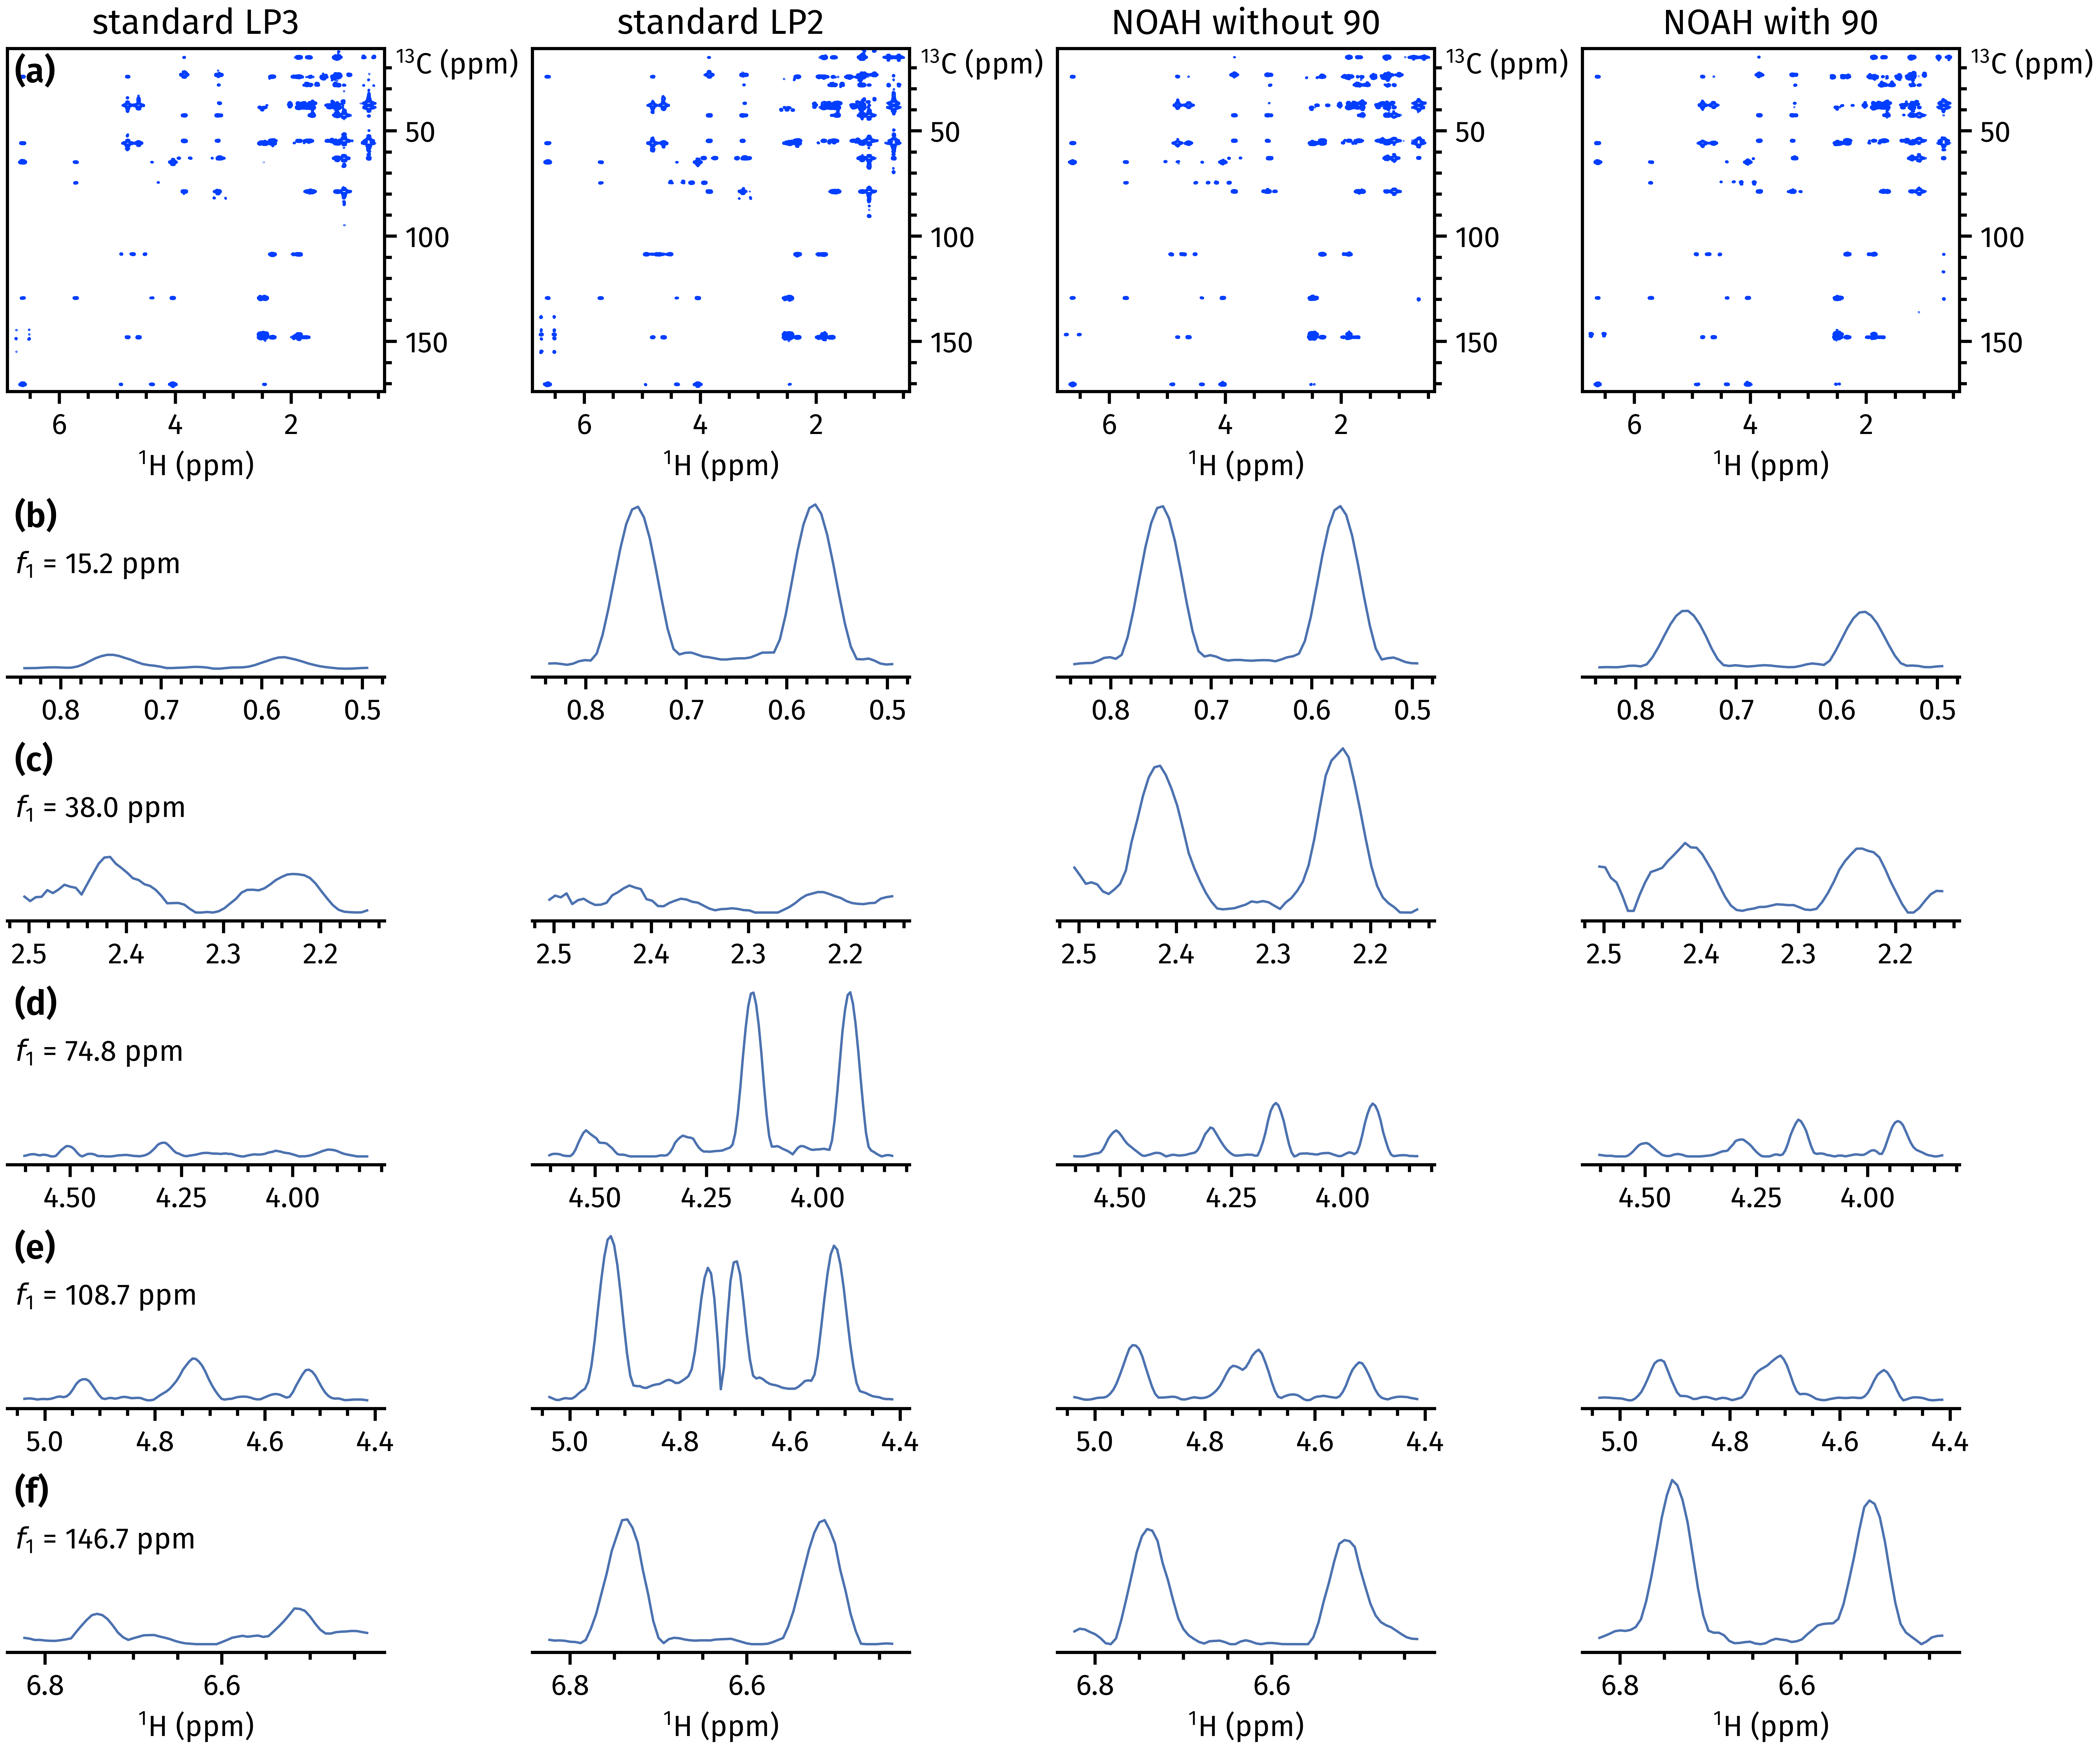
\includegraphics[width=\textwidth]{hmbc_si_andro.png}
    {\phantomsubcaption\label{fig:hmbc_si_andro_overall}}
    {\phantomsubcaption\label{fig:hmbc_si_andro_trace1}}
    {\phantomsubcaption\label{fig:hmbc_si_andro_trace2}}
    {\phantomsubcaption\label{fig:hmbc_si_andro_trace3}}
    {\phantomsubcaption\label{fig:hmbc_si_andro_trace4}}
    {\phantomsubcaption\label{fig:hmbc_si_andro_trace5}}
    \caption{
        Comparisons of HMBC spectra obtained using the Bruker standard library sequences\autocite{Cicero2001JMR} \texttt{hmbcetgpl3nd} (with a third-order LPJF, first column) and \texttt{hmbcetgpl2nd} (with a second-order LPJF, second column); and the NOAH \(zz\)-HMBC module (pulse sequence in \cref{fig:hmbc_comp_pulprog}), before and after the added \carbon{} \ang{90} pulse (third and fourth columns respectively).
        \textbf{(\subref{fig:hmbc_si_andro_overall})} The full 2D spectra, plotted with the same contour levels.
        \textbf{(\subref{fig:hmbc_si_andro_trace1})--(\subref{fig:hmbc_si_andro_trace5})} Multiple \(f_1\) traces through the 2D spectra showing the \(\onejch{}\) artefacts.
        Each row is plotted with the same \(y\)-axis range.
        In all cases except (\subref{fig:hmbc_si_andro_trace5}), the addition of the \ang{90} pulse leads to far better artefact suppression; in many cases, its performance is comparable to the standard library third-order LPJF.
        \andro{}
    }
    \label{fig:hmbc_si_andro}
\end{figure}

\begin{figure}[H]
    \centering
    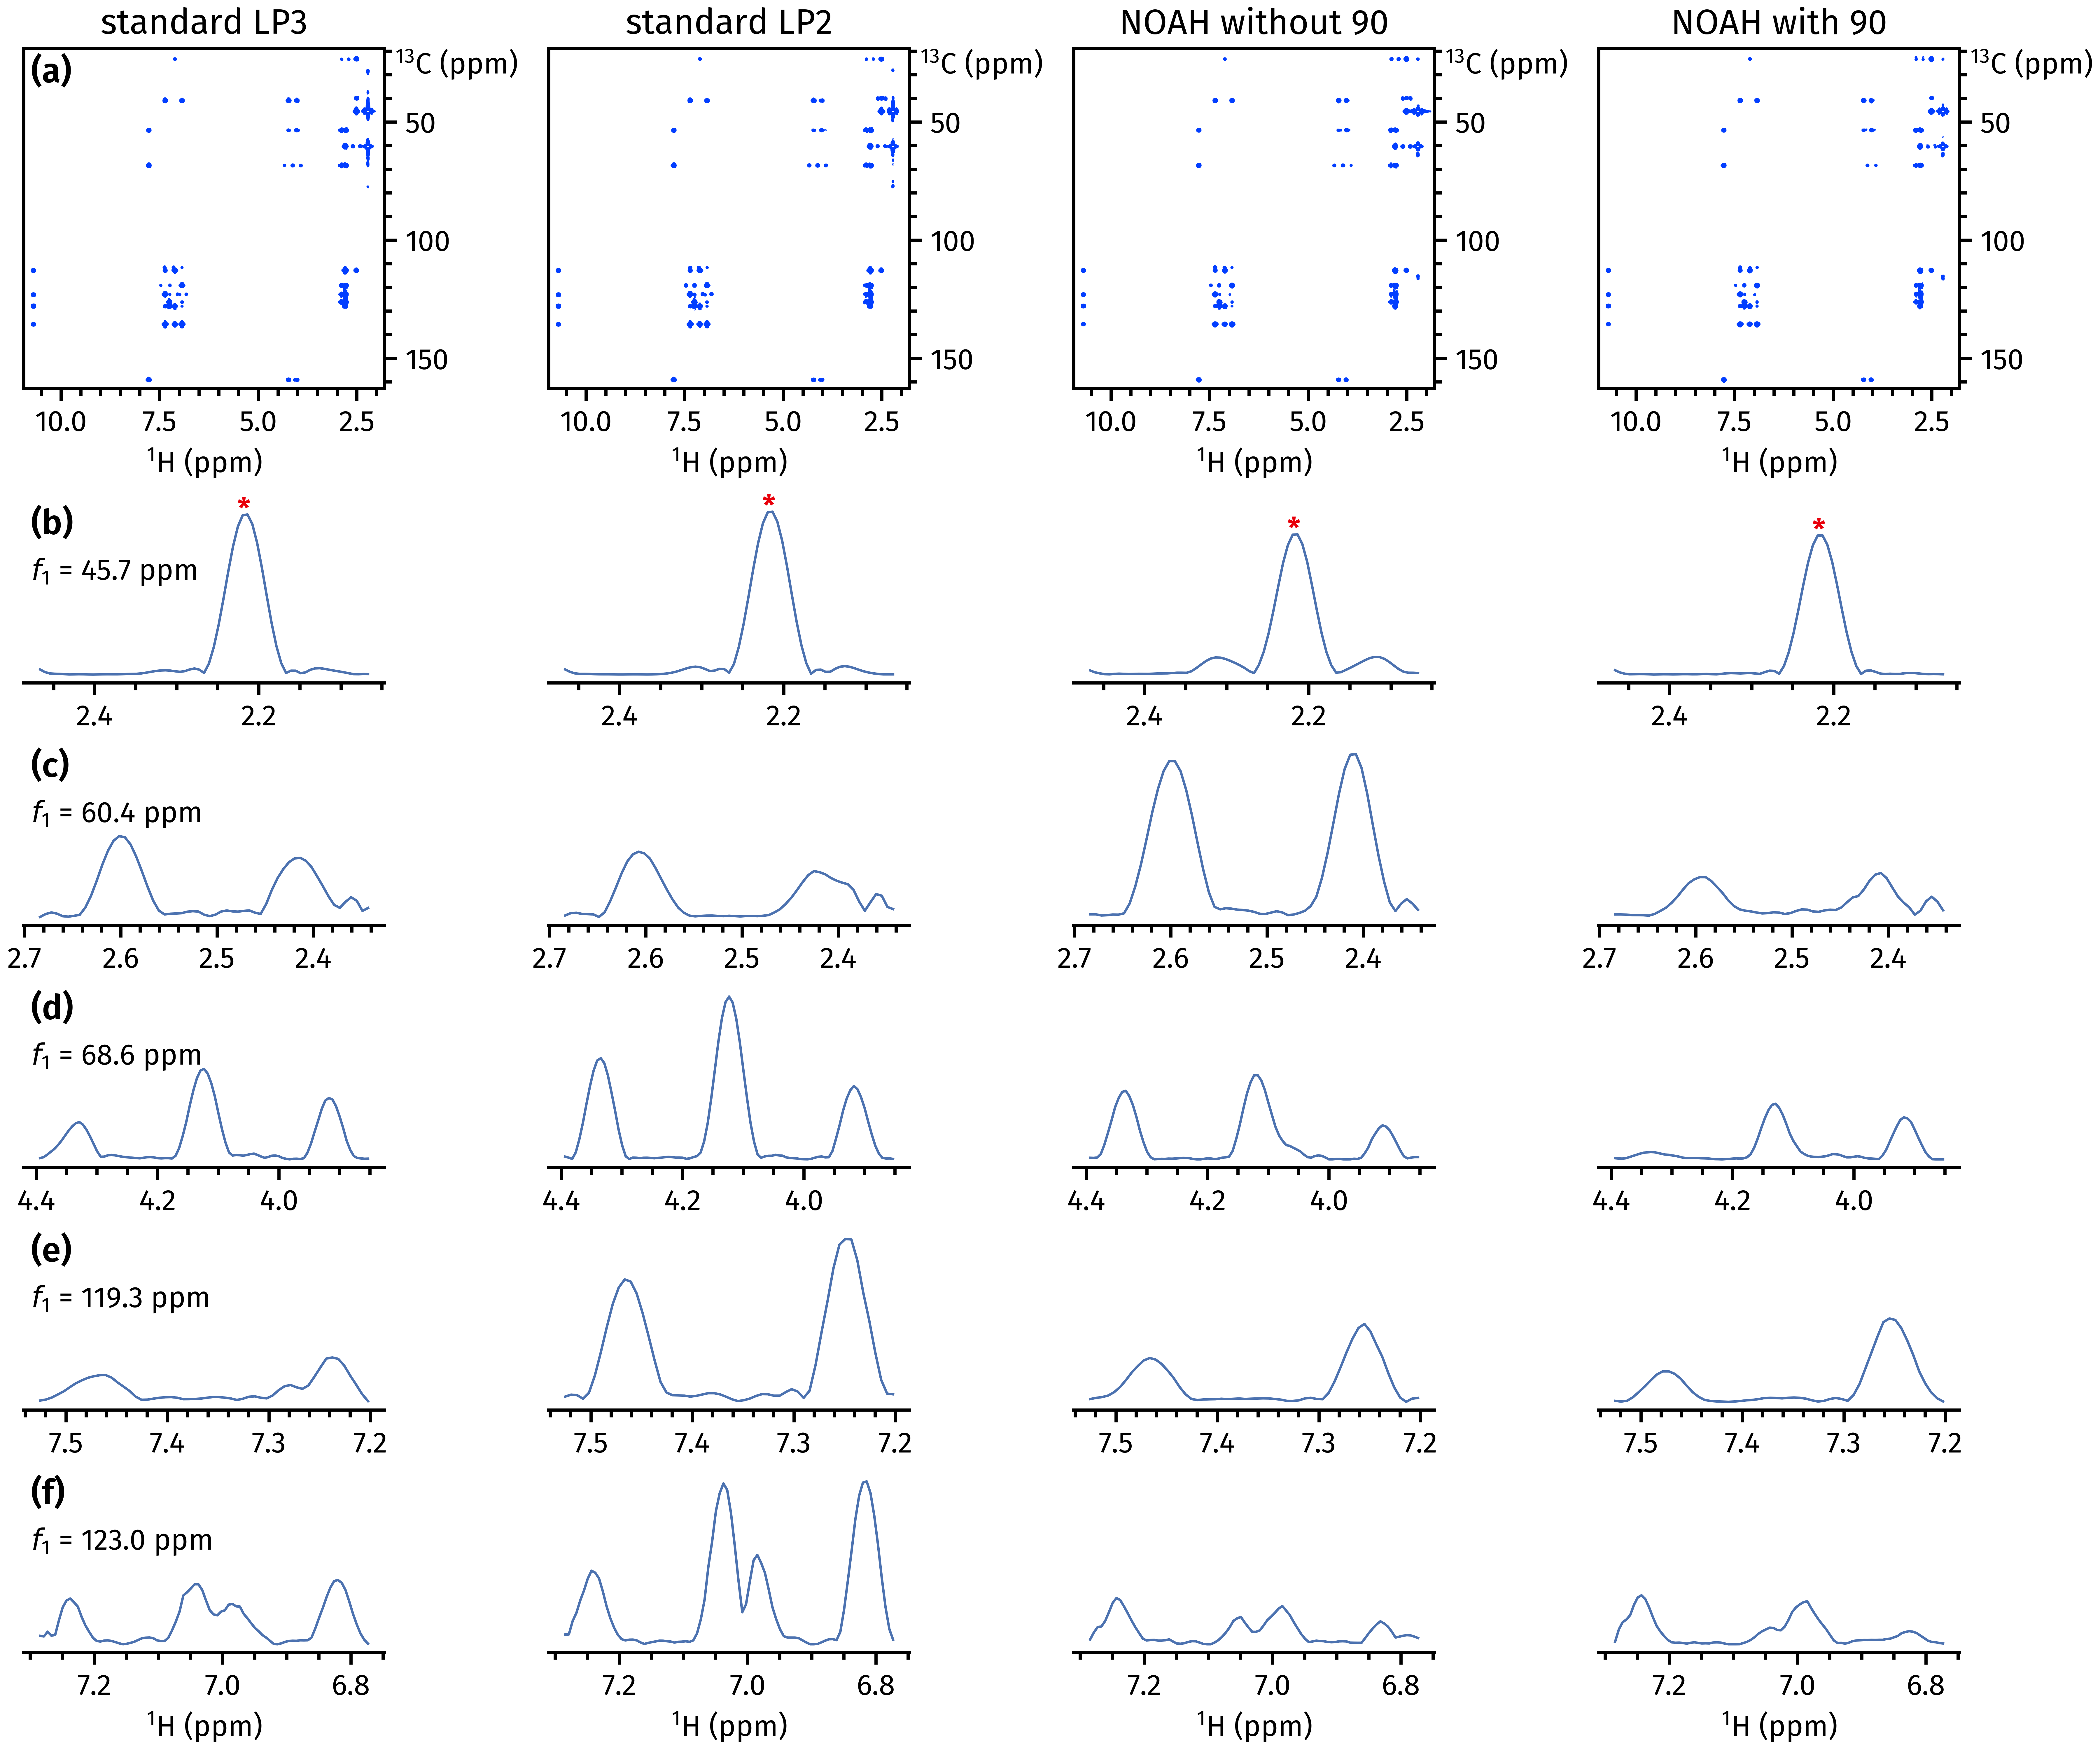
\includegraphics[width=\textwidth]{hmbc_si_zolmi.png}
    {\phantomsubcaption\label{fig:hmbc_si_zolmi_overall}}
    {\phantomsubcaption\label{fig:hmbc_si_zolmi_trace1}}
    {\phantomsubcaption\label{fig:hmbc_si_zolmi_trace2}}
    {\phantomsubcaption\label{fig:hmbc_si_zolmi_trace3}}
    {\phantomsubcaption\label{fig:hmbc_si_zolmi_trace4}}
    {\phantomsubcaption\label{fig:hmbc_si_zolmi_trace5}}
    \caption{
        The same as in \cref{fig:hmbc_si_andro}, but instead acquired with a sample of \SI{50}{\milli\molar} zolmitriptan in DMSO-\(d_6\).
        Note that the peak labelled with an asterisk in (\subref{fig:hmbc_si_zolmi_trace1}) is a genuine correlation.
        It is, however, flanked by a pair of \(\onejch{}\) artefacts (most visible in the third column, i.e.\ NOAH \(zz\)-HMBC without added \ang{90} pulse).
    }
    \label{fig:hmbc_si_zolmi}
\end{figure}

\section{HMQC sensitivity comparison}
\label{sec:si_hmqc_comp_snr}

\begin{figure}[H]
    \centering
    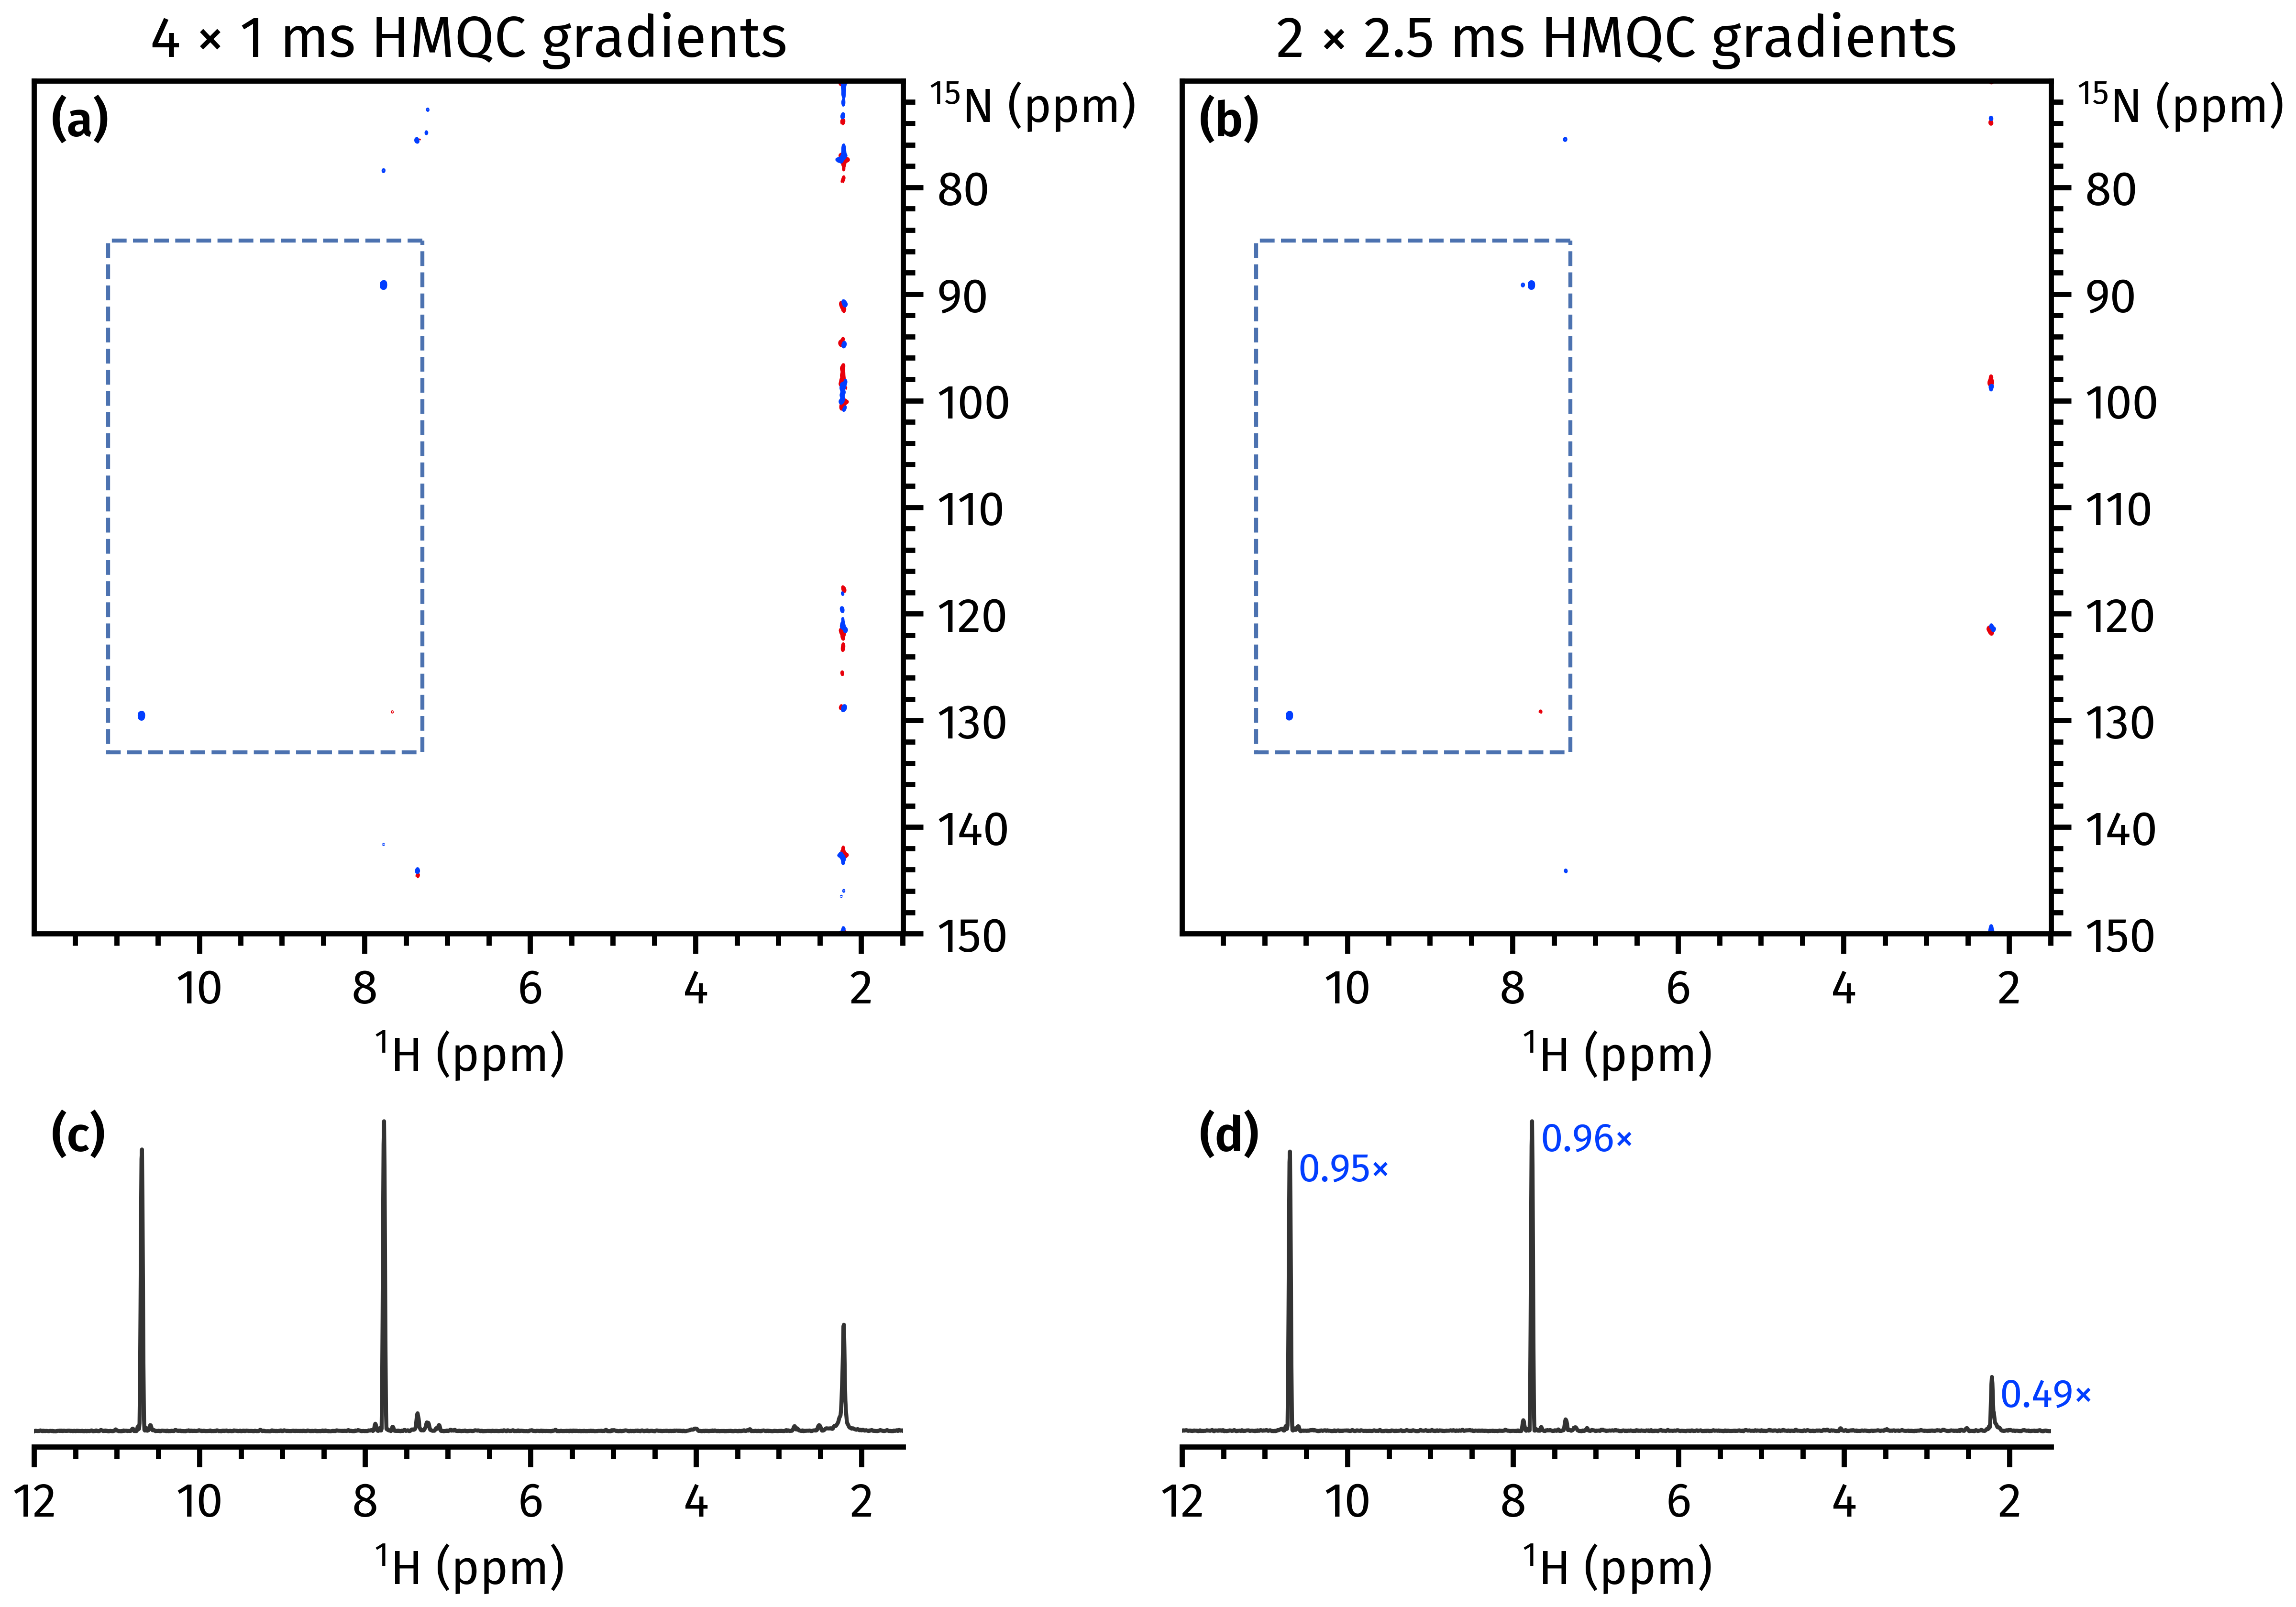
\includegraphics[width=0.8\textwidth]{hmqc_comp_snr.png}
    {\phantomsubcaption\label{fig:hmqc_comp_snr_bad2d}}
    {\phantomsubcaption\label{fig:hmqc_comp_snr_good2d}}
    {\phantomsubcaption\label{fig:hmqc_comp_snr_bad1d}}
    {\phantomsubcaption\label{fig:hmqc_comp_snr_good1d}}
    \caption{
        Comparisons of \HN{} HMQC spectra obtained using the two gradient schemes shown in \cref{fig:hmqc_comp}.
        \textbf{(\subref{fig:hmqc_comp_snr_bad2d})--(\subref{fig:hmqc_comp_snr_good2d})} Full 2D spectra.
        The two desired signals are boxed.
        Note the artefacts at \(f_2 = \SI{2.2}{\ppm}\); these arise from bulk magnetisation that is not fully dephased by the gradients in the HMQC module.
        \changed{These artefacts are also present in the standard Bruker HMQC / seHSQC sequences, and have comparable intensity to the unmodified NOAH spectrum in (\textbf{\subref{fig:hmqc_comp_snr_bad2d}}).\autocite{Yong2021JMR}}
        \textbf{(\subref{fig:hmqc_comp_snr_bad1d})--(\subref{fig:hmqc_comp_snr_good1d})} Positive projections of the spectra onto the \(f_2\) axis.
        The relative intensities of the peaks and artefacts are shown in (\subref{fig:hmqc_comp_snr_good1d}).
        Switching to the improved gradient scheme leads to no significant change in the intensity of the desired peaks (\(\geq 95\%\)), and halves the artefact intensity.
        We previously reported similar results with the \HN{} seHSQC module.\autocite{Yong2021JMR}
        \zolmi{}
    }
    \label{fig:hmqc_comp_snr}
\end{figure}

% Fakesection SI bibliography
\printbibliography{}
\end{refsection}

\end{document}
